\documentclass[conference]{IEEEtran}
\usepackage[T1]{fontenc}
\usepackage{cite}
\usepackage{amsmath,amssymb}
\usepackage{graphicx}
\usepackage{booktabs}
\usepackage{array}
\usepackage{url}
\usepackage{hyperref}
\graphicspath{{figures/}}
\hypersetup{colorlinks=true,linkcolor=black,citecolor=black,urlcolor=blue}

\begin{document}

\title{Automatic Clothing Category Recognition:\\ Handcrafted Features versus Raw Pixels with Classical Machine Learning\\ (Phase 1 --- Machine-Learning Evaluation)}

\author{\IEEEauthorblockN{Team Member 1, Sibtain Ahmed Qureshi, Team Member 3}
\IEEEauthorblockA{Department of Computer Science / Applied Machine Learning\\
Institution Name\\
Emails: \texttt{sibtainahmedqureshi28@gmail.com}}}

\maketitle

\begin{abstract}
We study automatic tagging of clothing images for a small catalogue using the Fashion-MNIST benchmark (70{,}000 grayscale $28\times28$ images, 10 classes). Phase~1 asks whether a fixed image descriptor, the Histogram of Oriented Gradients (HOG), improves classical classifiers over flattened pixels. We compare Logistic Regression, $k$-Nearest Neighbours, Random Forest and an RBF Support Vector Machine on three representations (raw pixels, HOG, HOG plus 16 shape statistics) under a strict protocol: the official train/test split is preserved, a stratified validation set is drawn only from the training data, hyper-parameters are tuned on validation, and the test set is used once. HOG improves three of four classifiers significantly (McNemar $p<0.001$): +4.0 points for Logistic Regression, +2.1 for $k$-NN and +1.4 for SVM, whereas Random Forest is unchanged (+0.2, $p=0.49$). The best model, an RBF SVM on HOG, reaches 91.3\% test accuracy and 0.913 macro-F1. About 60--65\% of all errors of every model stay inside the group \{T-shirt, Pullover, Coat, Shirt\}, and Shirt recall is only 0.75, which motivates the CNN studied in Phase~2.
\end{abstract}

\begin{IEEEkeywords}
Fashion-MNIST, HOG, feature engineering, support vector machine, random forest, k-nearest neighbours, logistic regression, error analysis
\end{IEEEkeywords}

%=====================================================================
\section{Introduction}
Online retailers and small shops maintain catalogues in which every product image must carry a category tag. Manual tagging is slow and inconsistent, so an automatic classifier is attractive. Fashion-MNIST~\cite{xiao2017} was proposed as a drop-in, harder replacement for the digit benchmark MNIST~\cite{lecun1998}: the images have the same format but represent clothing, and simple classifiers no longer saturate.

\textbf{Problem statement.} Given a $28\times28$ grayscale image, predict one of ten categories. The project has two phases. Phase~1 (this report) covers the classical machine-learning part: a baseline of flattened pixels and HOG descriptors with four classical learners. Phase~2 will add a small convolutional neural network (CNN) and compare it with Phase~1.

\textbf{Gap addressed.} Flattening an image into a vector discards the 2-D neighbourhood structure, while HOG fixes the representation (local gradient orientations) before the model has seen any category-specific example. It is therefore not obvious which choice is better for which learner, nor at what cost in model size and inference time.

\textbf{Contributions.}
\begin{enumerate}
\item A structured data-quality audit and EDA that predicts which classes will be confused (Section~\ref{sec:eda}).
\item A feature-engineering study with a HOG hyper-parameter ablation, 16 interpretable shape statistics and PCA (Section~\ref{sec:fe}).
\item A fair, fully reproducible comparison of $4\times3$ model/feature configurations with accuracy, macro-F1, per-class recall, parameter count and latency (Section~\ref{sec:results}).
\item Statistical validation (McNemar test, bootstrap confidence intervals) and an error analysis of the upper-body garment group (Section~\ref{sec:errors}).
\end{enumerate}

%=====================================================================
\section{Literature Review}
\textbf{Benchmark.} Xiao et al.~\cite{xiao2017} released Fashion-MNIST with 60{,}000 training and 10{,}000 test images from Zalando articles, converted to $28\times28$ grayscale, and benchmarked 129 classifier configurations from scikit-learn. They report that tree ensembles and SVMs on raw pixels reach the high 80s to about 90\%, and that the shirt-like classes are the hardest. LeCun et al.~\cite{lecun1998} established the MNIST protocol and showed that convolutional networks trained with gradient-based learning outperform fixed feature extractors on digits.

\textbf{Handcrafted descriptors.} Dalal and Triggs~\cite{dalal2005} introduced HOG for pedestrian detection: image gradients are binned by orientation inside small cells and normalised over overlapping blocks, giving robustness to local illumination and small shifts. Related descriptors include SIFT~\cite{lowe2004} and Local Binary Patterns~\cite{ojala2002}. For small $28\times28$ inputs the choice of cell size is critical, because a classic $8\times8$ cell would cover almost a third of the image.

\textbf{Classical learners.} Logistic Regression is the standard linear probabilistic classifier~\cite{hastie2009}. $k$-NN~\cite{cover1967} is non-parametric and stores the training set. Random Forests~\cite{breiman2001} average decorrelated decision trees. Support Vector Machines~\cite{cortes1995} maximise the margin and, with an RBF kernel, learn non-linear boundaries with implicit infinite-dimensional features.

\textbf{Dimensionality reduction and visualisation.} PCA~\cite{jolliffe2002} and t-SNE~\cite{vandermaaten2008} are used in the EDA to measure redundancy and inspect class overlap.

\textbf{Evaluation methodology.} Because all classifiers are scored on the same 10{,}000 test images, paired tests are appropriate; McNemar's test~\cite{mcnemar1947} on discordant pairs is recommended by Dietterich~\cite{dietterich1998} for single-split comparisons. The bootstrap~\cite{efron1979} provides confidence intervals.

\textbf{Positioning.} Prior work either reports raw-pixel baselines or CNNs. Our study isolates the effect of a \emph{fixed} descriptor on four learner families, with equal tuning budget, a clean validation protocol and costs (parameters, latency) reported next to accuracy.

%=====================================================================
\section{Dataset Quality and Exploratory Data Analysis}\label{sec:eda}
\subsection{Data description and audit}
The raw IDX files are read with \texttt{gzip} and \texttt{numpy.frombuffer} (\texttt{src/data\_loader.py}). Table~\ref{tab:quality} lists the audit performed by \texttt{eda.quality\_report}.

\begin{table}[t]
\centering\caption{Data-quality audit.}\label{tab:quality}
\begin{tabular}{@{}ll@{}}\toprule
Check & Result\\\midrule
Train / test shape & $(60000,28,28)$ / $(10000,28,28)$\\
dtype, range & uint8, $[0,255]$\\
Missing values & 0\\
Blank images & 0\\
Exact duplicates (train) & 0\\
Train--test overlap & 0\\
Duplicate images with different labels & 0\\
Zero-valued pixels & 50.2\%\\
Mean / std of pixel (scaled) & 0.286 / 0.353\\\bottomrule
\end{tabular}\end{table}

The data are clean, so no imputation, removal or de-duplication is required. The only preprocessing step is the scaling $x\leftarrow x/255$. Labels are never altered.

\subsection{Class balance and split shift}
Every class has exactly 6{,}000 training and 1{,}000 test images (Fig.~\ref{fig:class}). Accuracy is therefore meaningful, but we still report macro-F1 and per-class recall. A two-sample Kolmogorov--Smirnov test on the per-image mean intensity finds no train/test shift ($D=0.0064$, $p=0.87$); the largest mean-pixel difference is 0.0086.

\begin{figure}[t]\centering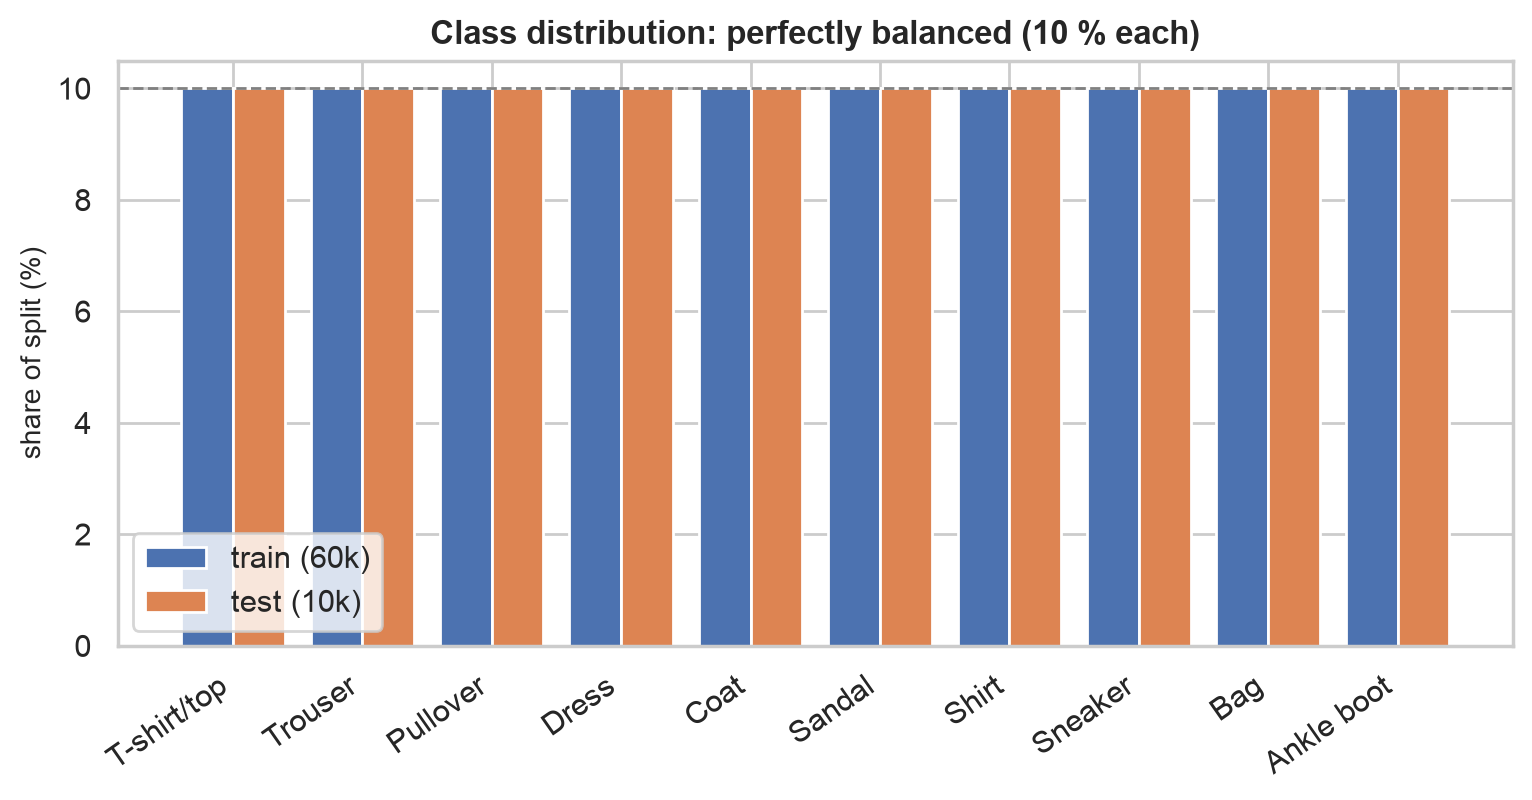
\includegraphics[width=\columnwidth]{eda_01_class_distribution.png}\caption{Balanced classes in both splits.}\label{fig:class}\end{figure}

\subsection{Visual and intensity analysis}
Fig.~\ref{fig:samples} shows random samples and Fig.~\ref{fig:mean} the per-class mean and standard-deviation images. Footwear classes have small bounding-box height and large width (Sandal mean width 27.8~px, height 16.1~px; Sneaker height 13.4~px), Trouser is narrow (11.7~px), and the four upper-body classes have almost identical extents ($\approx$21~px wide, $\approx$28~px high). The pixel-level standard deviation is highest at garment edges and sleeves. Fig.~\ref{fig:box} shows the distribution of brightness, ink coverage and width.

\begin{figure}[t]\centering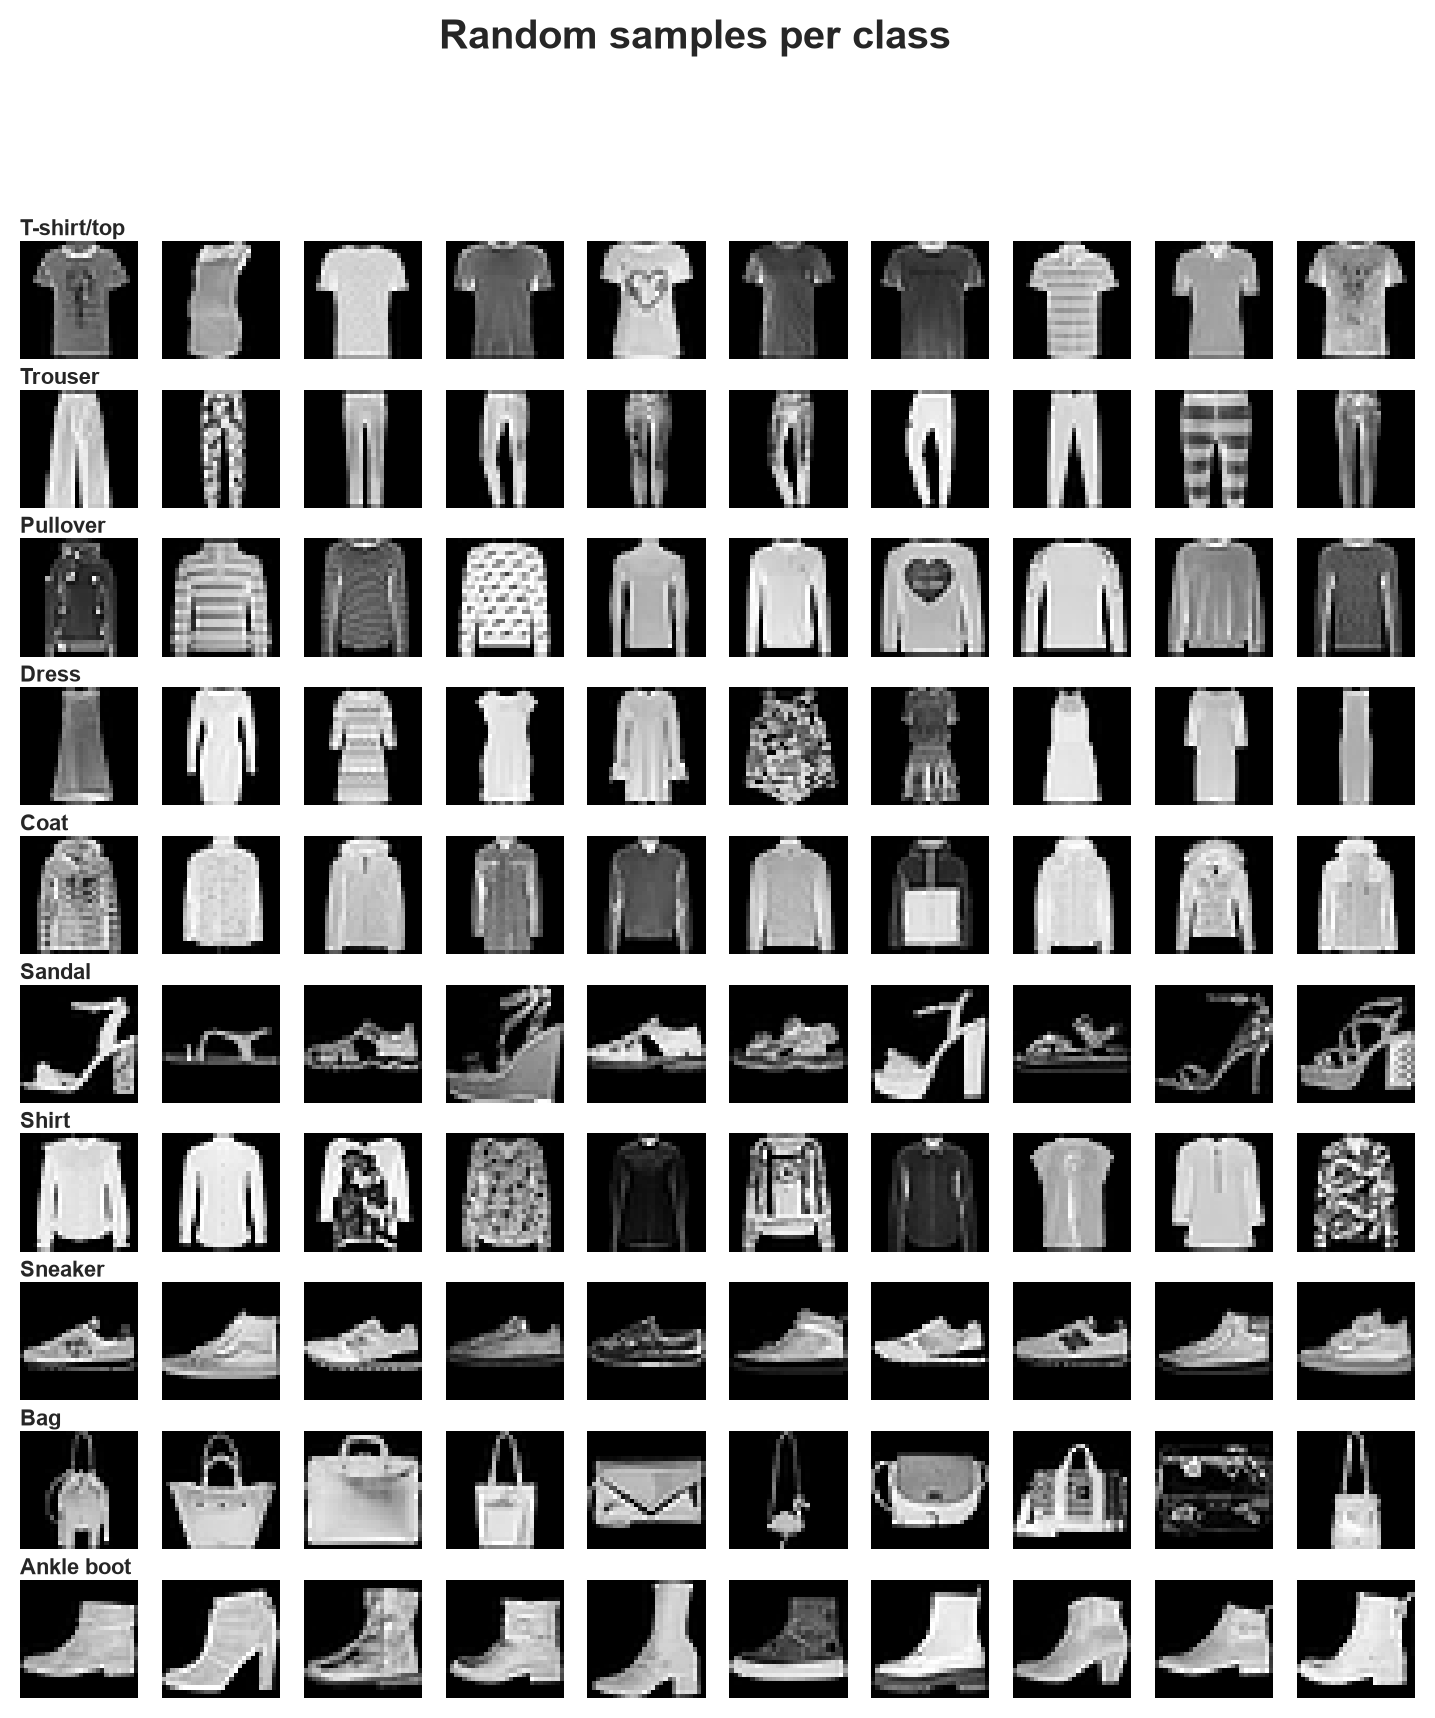
\includegraphics[width=\columnwidth]{eda_02_sample_grid.png}\caption{Random samples per class.}\label{fig:samples}\end{figure}
\begin{figure*}[t]\centering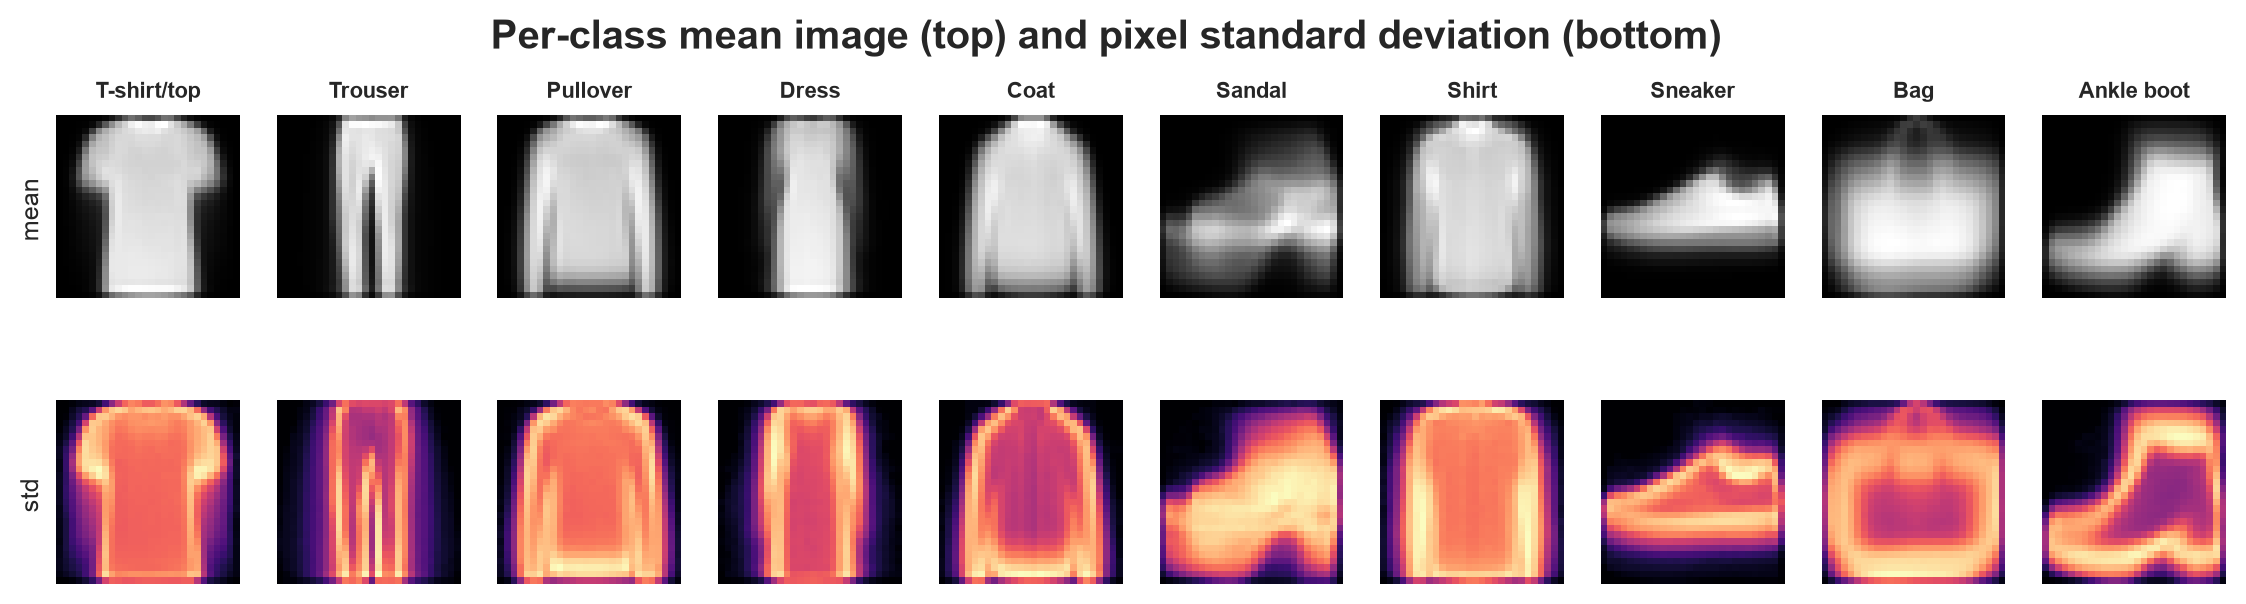
\includegraphics[width=\textwidth]{eda_03_mean_std_images.png}\caption{Class-mean (top) and pixel standard-deviation (bottom) images.}\label{fig:mean}\end{figure*}
\begin{figure*}[t]\centering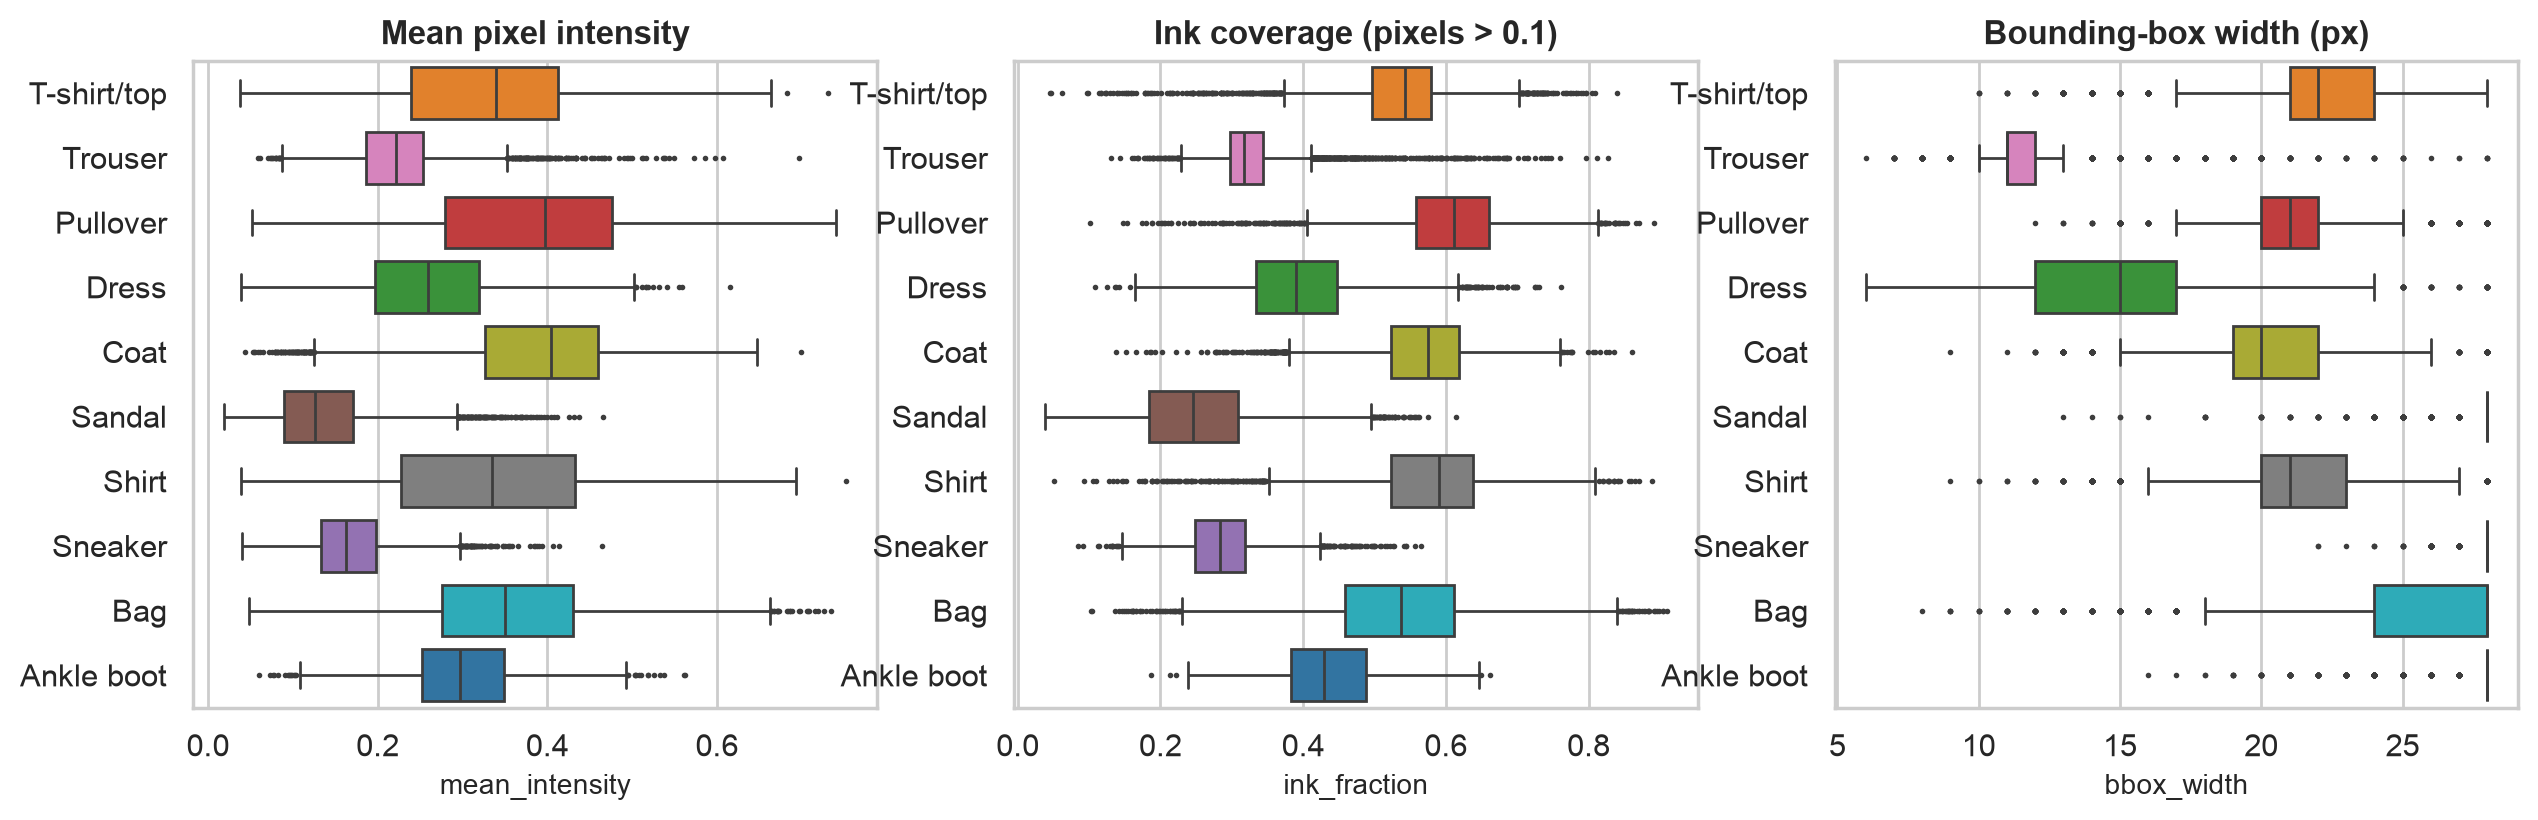
\includegraphics[width=\textwidth]{eda_04_intensity_shape_boxplots.png}\caption{Per-class distributions of mean intensity, ink coverage and bounding-box width.}\label{fig:box}\end{figure*}

\subsection{Pixel relevance and spatial structure}
\texttt{sklearn.feature\_selection.f\_classif} gives an ANOVA F-score per pixel; together with the pixel variance (Fig.~\ref{fig:fscore}) it shows that 31 border pixels have variance below $10^{-3}$ and carry no information. We then compute the mean Pearson correlation between pixel pairs as a function of their distance (Fig.~\ref{fig:corr}): adjacent pixels correlate at $r\approx0.75$, decaying to $0.09$ at 14~px, whereas the same pixels with shuffled positions stay at $r\approx0.16$. Neighbourhood structure is therefore real and is ignored by flattening, which is the empirical motivation for HOG.

\begin{figure}[t]\centering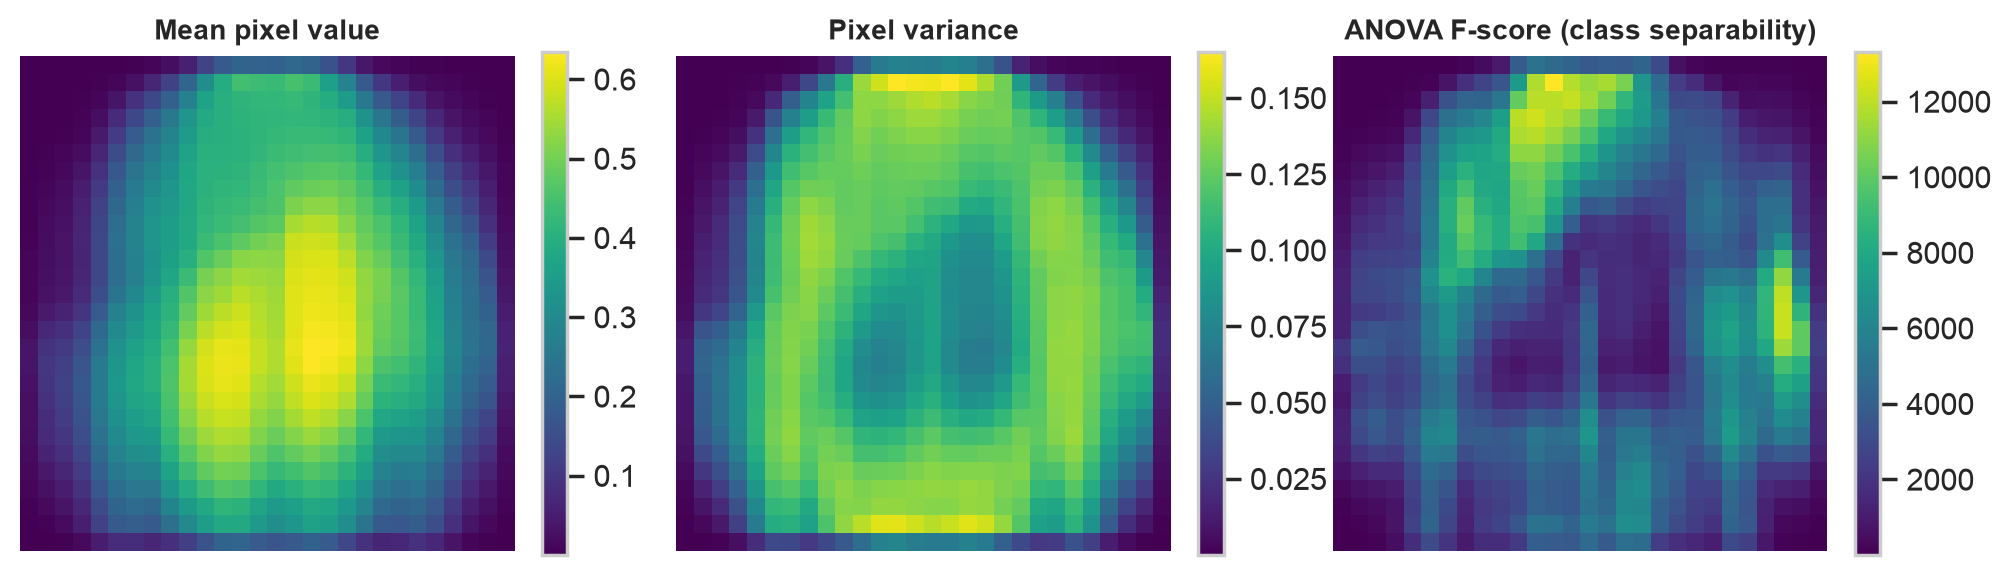
\includegraphics[width=\columnwidth]{eda_06_pixel_variance_fscore.png}\caption{Mean, variance and F-score per pixel.}\label{fig:fscore}\end{figure}
\begin{figure}[t]\centering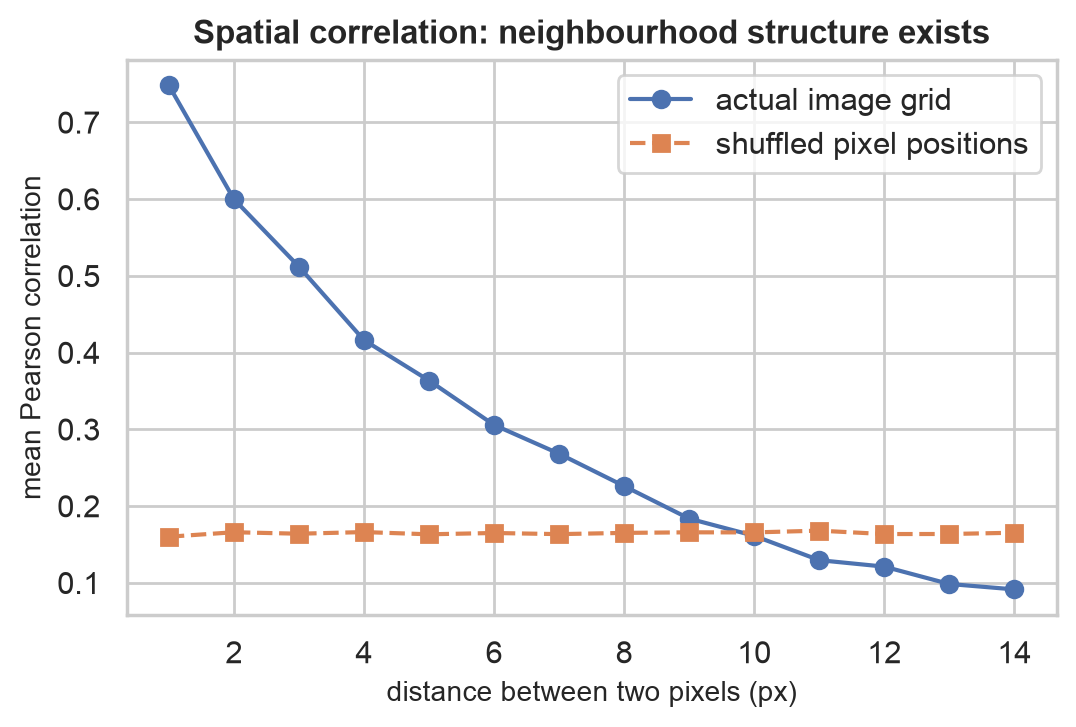
\includegraphics[width=0.85\columnwidth]{eda_07_spatial_correlation.png}\caption{Pixel correlation versus distance.}\label{fig:corr}\end{figure}

\subsection{Class similarity, PCA and t-SNE}
The Euclidean distance between class-mean images (Fig.~\ref{fig:dist}) ranks the closest pairs: Pullover--Coat (2.48), Pullover--Shirt (2.68), Coat--Shirt (3.02), T-shirt--Shirt (3.72). Sandal--Sneaker (3.84) is the only non-upper-body pair in this group. This \emph{predicts} the confusion structure later observed in Section~\ref{sec:errors}.

PCA on pixels (Fig.~\ref{fig:pca}) needs 24, 84 and 187 components to retain 80\%, 90\% and 95\% of the variance, i.e.\ the 784 pixels are highly redundant. t-SNE on 5{,}000 images after PCA-50 (Fig.~\ref{fig:tsne}) shows compact clusters for Trouser, Bag and footwear and a large overlap among the upper-body classes. Fig.~\ref{fig:amb} lists examples of that ambiguous group.

\begin{figure}[t]\centering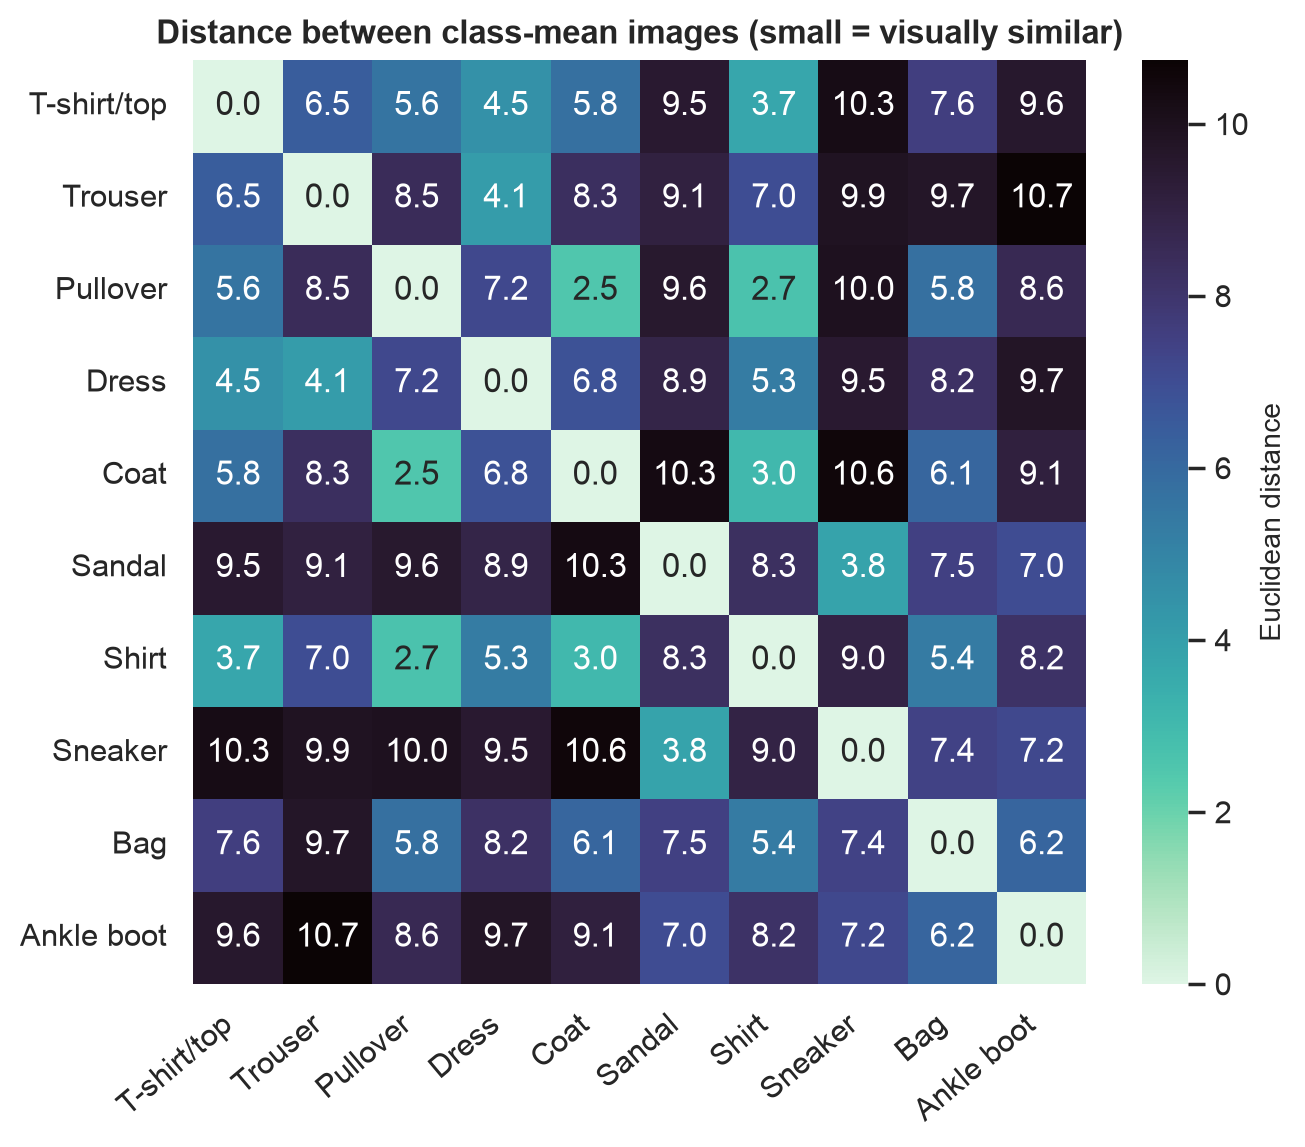
\includegraphics[width=\columnwidth]{eda_08_class_mean_distance.png}\caption{Distance between class-mean images.}\label{fig:dist}\end{figure}
\begin{figure*}[t]\centering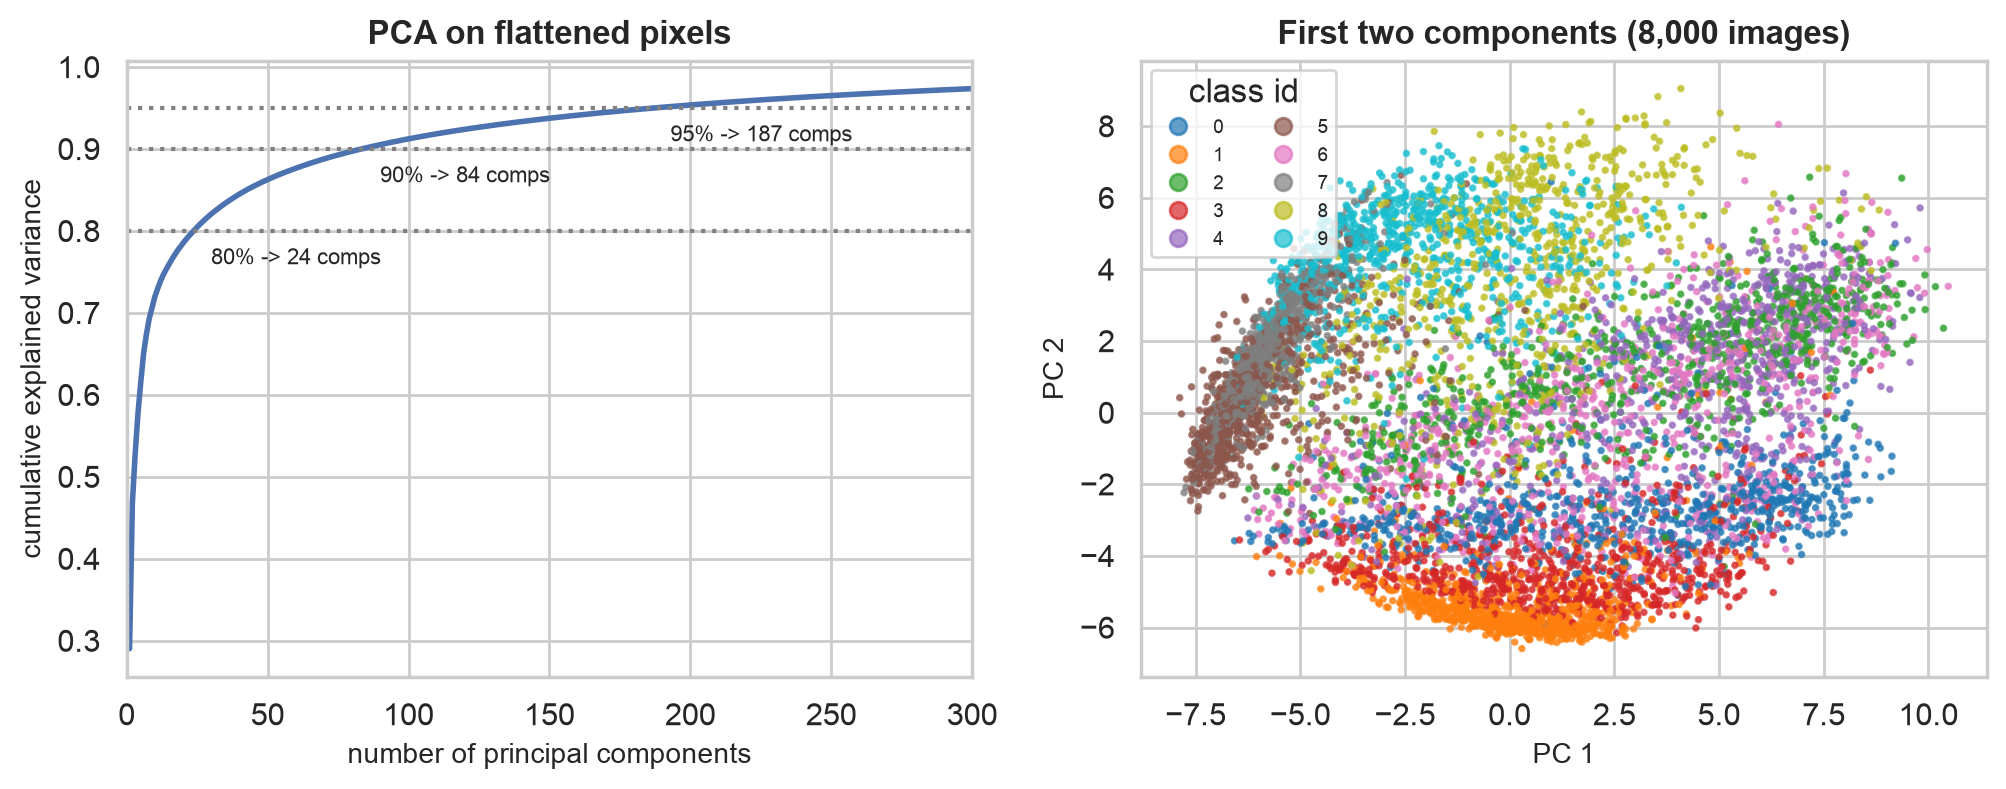
\includegraphics[width=\textwidth]{eda_09_pca.png}\caption{PCA: cumulative variance and first two components.}\label{fig:pca}\end{figure*}
\begin{figure}[t]\centering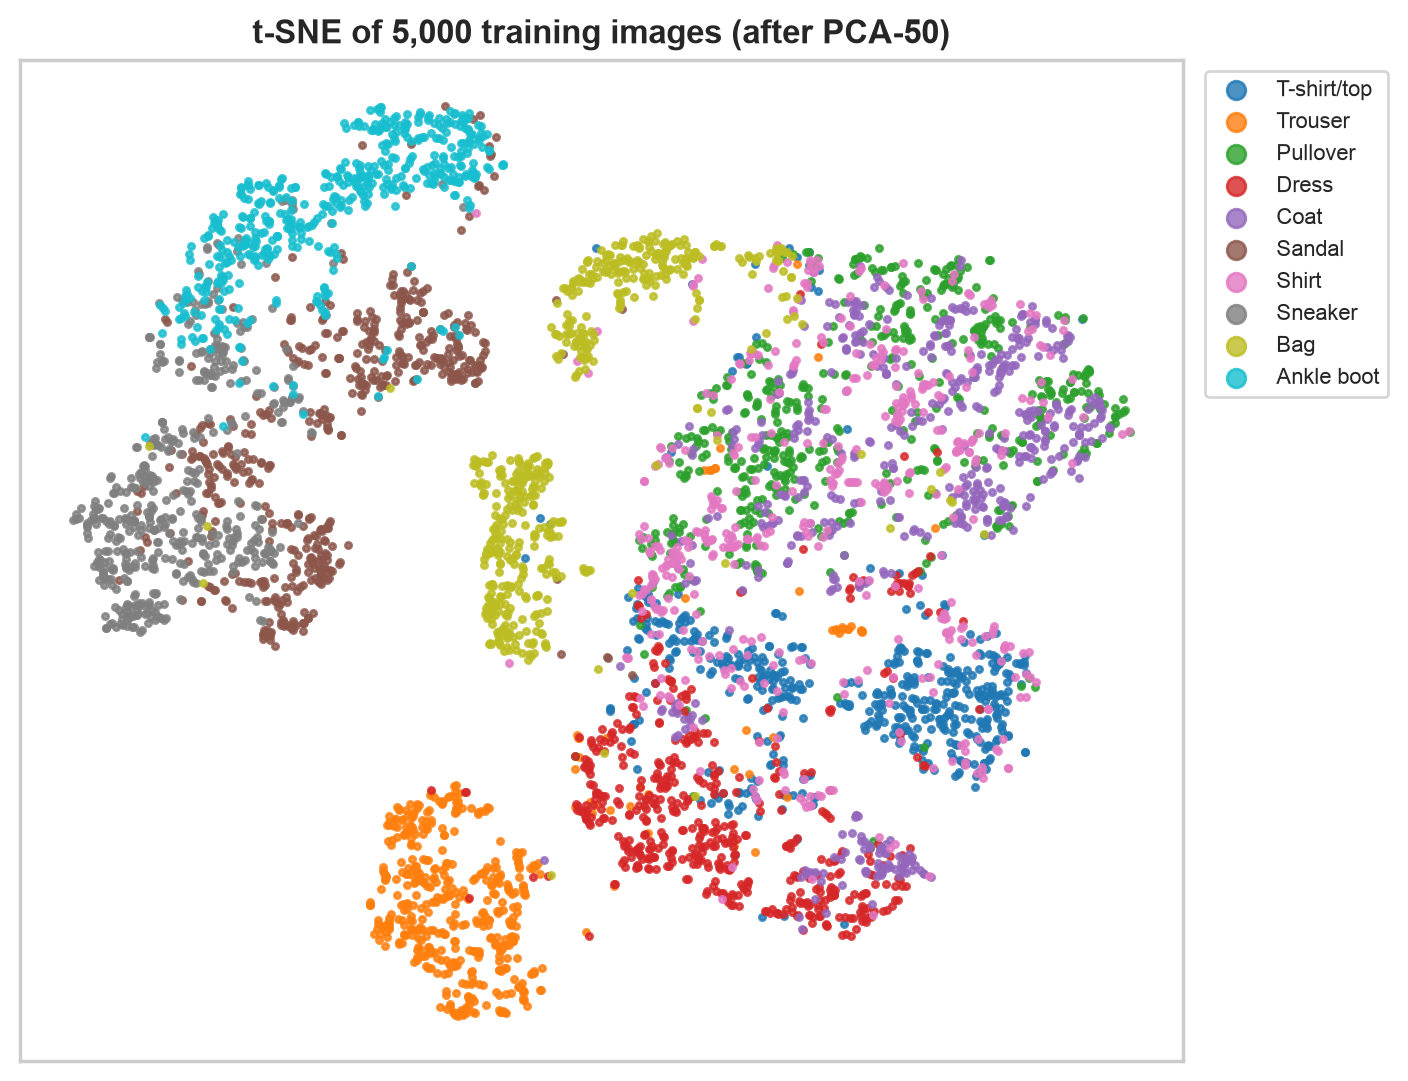
\includegraphics[width=\columnwidth]{eda_10_tsne.png}\caption{t-SNE of 5{,}000 training images.}\label{fig:tsne}\end{figure}
\begin{figure}[t]\centering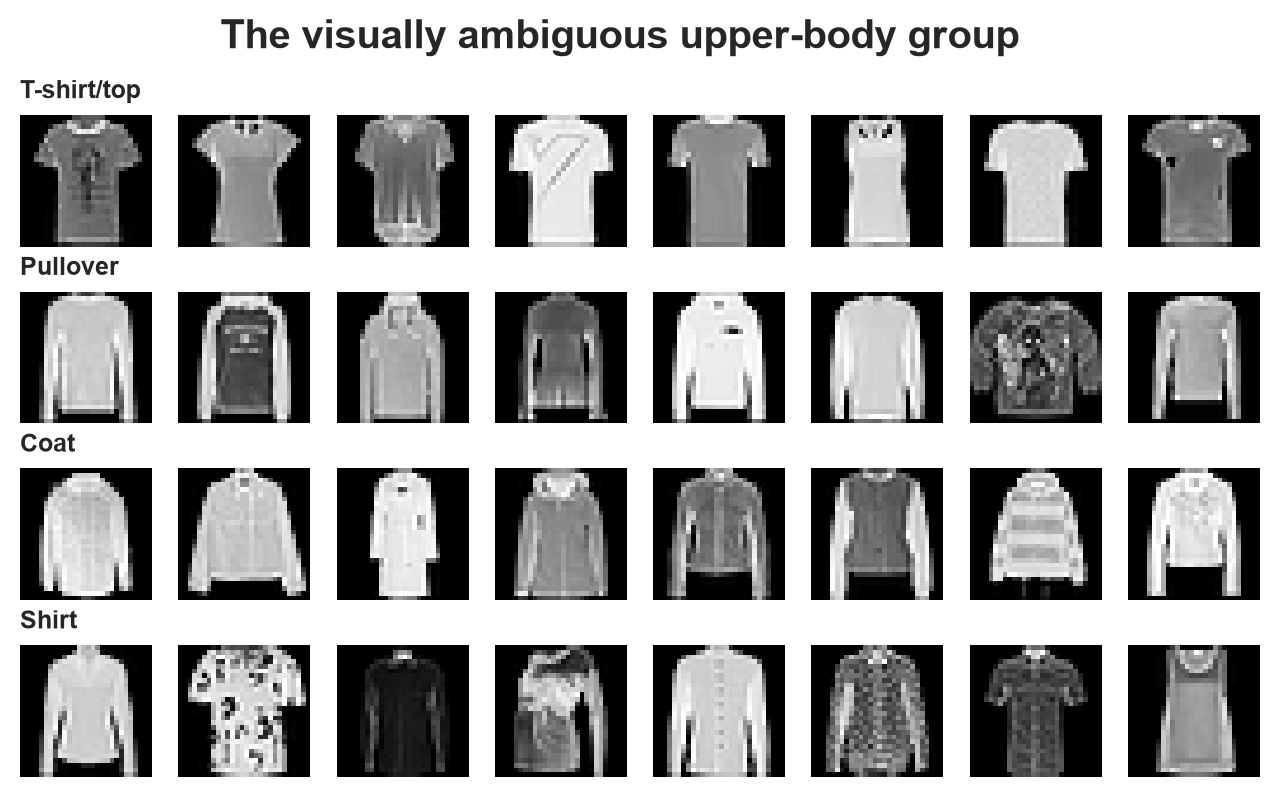
\includegraphics[width=\columnwidth]{eda_12_ambiguous_group.png}\caption{Upper-body garments: T-shirt/top, Pullover, Coat, Shirt.}\label{fig:amb}\end{figure}

\subsection{Orientation check}
HOG is orientation-sensitive, so we verified image orientation. The mean top-minus-bottom ink share is positive for T-shirt (+0.08) and Trouser (+0.15) and strongly negative for Sandal, Sneaker, Bag and Ankle boot ($\approx -0.3$), consistent with upright garments and footwear soles at the bottom. Images are stored row-major, upright, so HOG is applied directly with no rotation.

%=====================================================================
\section{Feature Engineering}\label{sec:fe}
Three feature sets are built by \texttt{src/features.py}.

\subsection{Raw pixels (784-d)}
\texttt{flatten\_pixels} reshapes the $28\times28$ image in row-major order after scaling to $[0,1]$.

\subsection{Histogram of Oriented Gradients}
HOG~\cite{dalal2005} is computed with \texttt{skimage.feature.hog}. For each pixel the gradients $g_x,g_y$ give magnitude $m=\sqrt{g_x^2+g_y^2}$ and orientation $\theta=\operatorname{atan2}(g_y,g_x)$ (unsigned, $[0^\circ,180^\circ)$). The image is divided into cells of $p\times p$ pixels; each cell accumulates a histogram of $B$ orientation bins weighted by $m$. Cells are grouped into overlapping blocks of $2\times2$ cells and each block vector $v$ is normalised with L2-Hys ($v\leftarrow v/\sqrt{\|v\|_2^2+\epsilon^2}$, clip at 0.2, renormalise). The descriptor is the concatenation of all block vectors. For an $n\times n$ image with $c=n/p$ cells per side the length is $(c-1)^2\cdot4\cdot B$. Fig.~\ref{fig:hogvis} visualises the descriptor. Extraction is parallelised with \texttt{joblib.Parallel}.

\begin{figure*}[t]\centering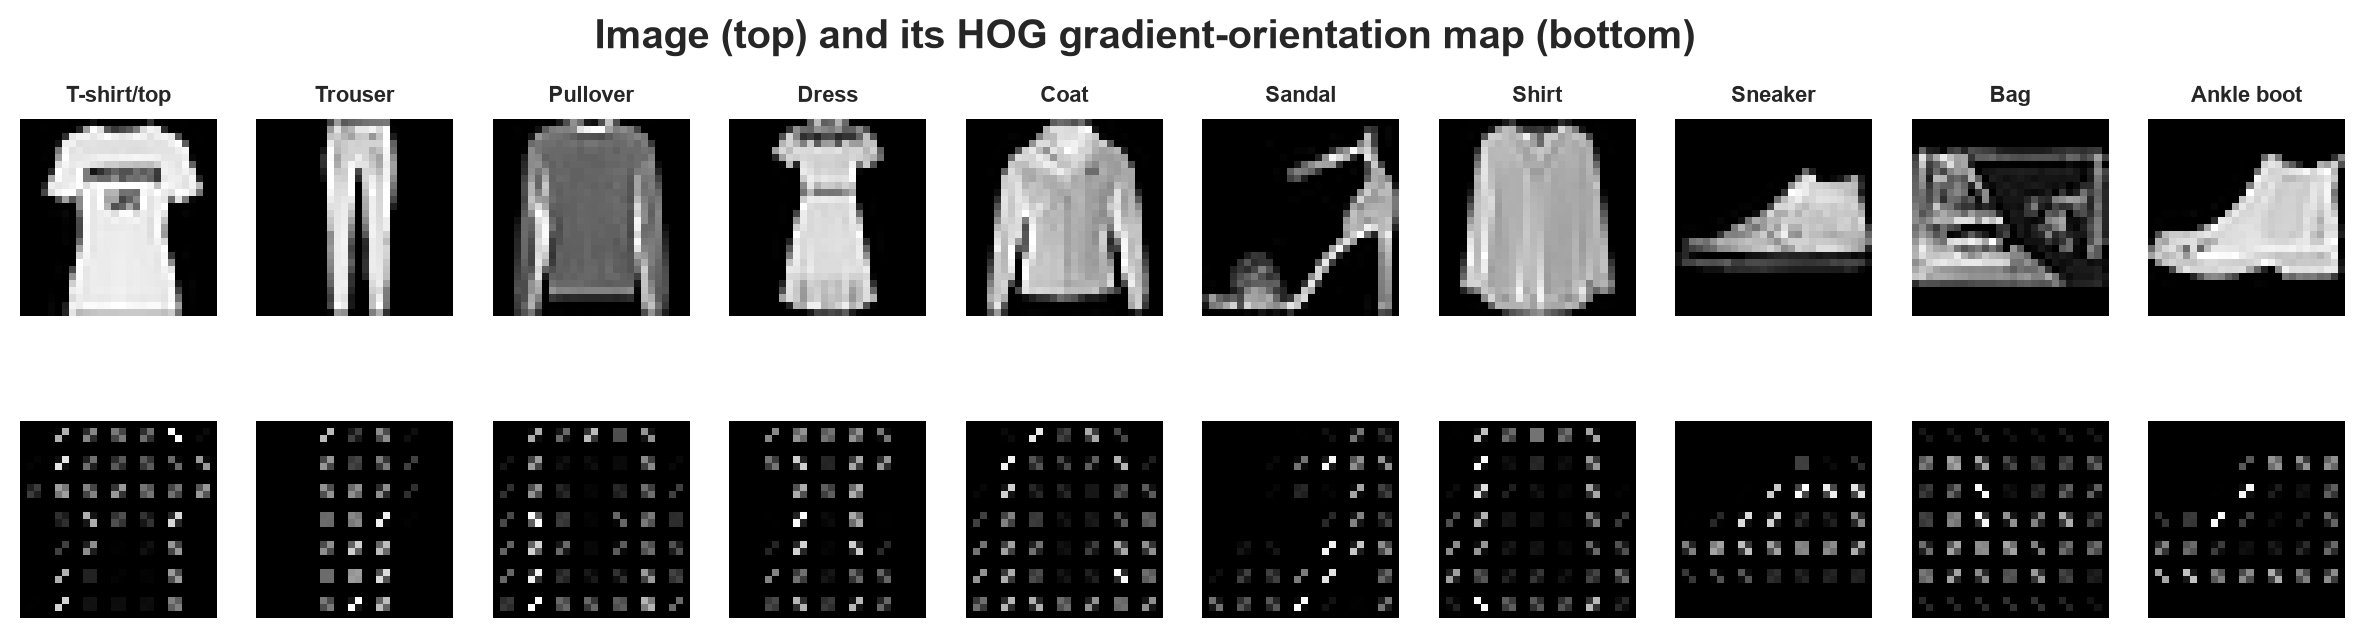
\includegraphics[width=\textwidth]{fe_02_hog_visual.png}\caption{Images and the HOG orientation map for one example per class.}\label{fig:hogvis}\end{figure*}

\textbf{Ablation.} We evaluated $B\in\{6,9,12\}$, cell size $\in\{2,4,7\}$ and block size $\in\{1,2\}$ cells (36 configurations) with a fast Logistic-Regression probe (\texttt{StandardScaler}, $C=0.5$) trained on 12{,}000 images and scored on the validation set (Fig.~\ref{fig:hogab}). Small cells win (best: $B=12$, $2\times2$ cells, $2\times2$ blocks, 0.870 but 8{,}112-d), and $2\times2$ blocks beat $1\times1$. Since kNN, SVM and RF scale with dimensionality, we select the best configuration with at most 2{,}000 dimensions: $B=6$, $4\times4$ cells, $2\times2$ blocks, \textbf{864-d} (probe accuracy 0.856). This \emph{a priori} fixed descriptor is then used by all four classifiers, matching the project premise that HOG fixes the representation before the model sees category-specific examples.

\begin{figure*}[t]\centering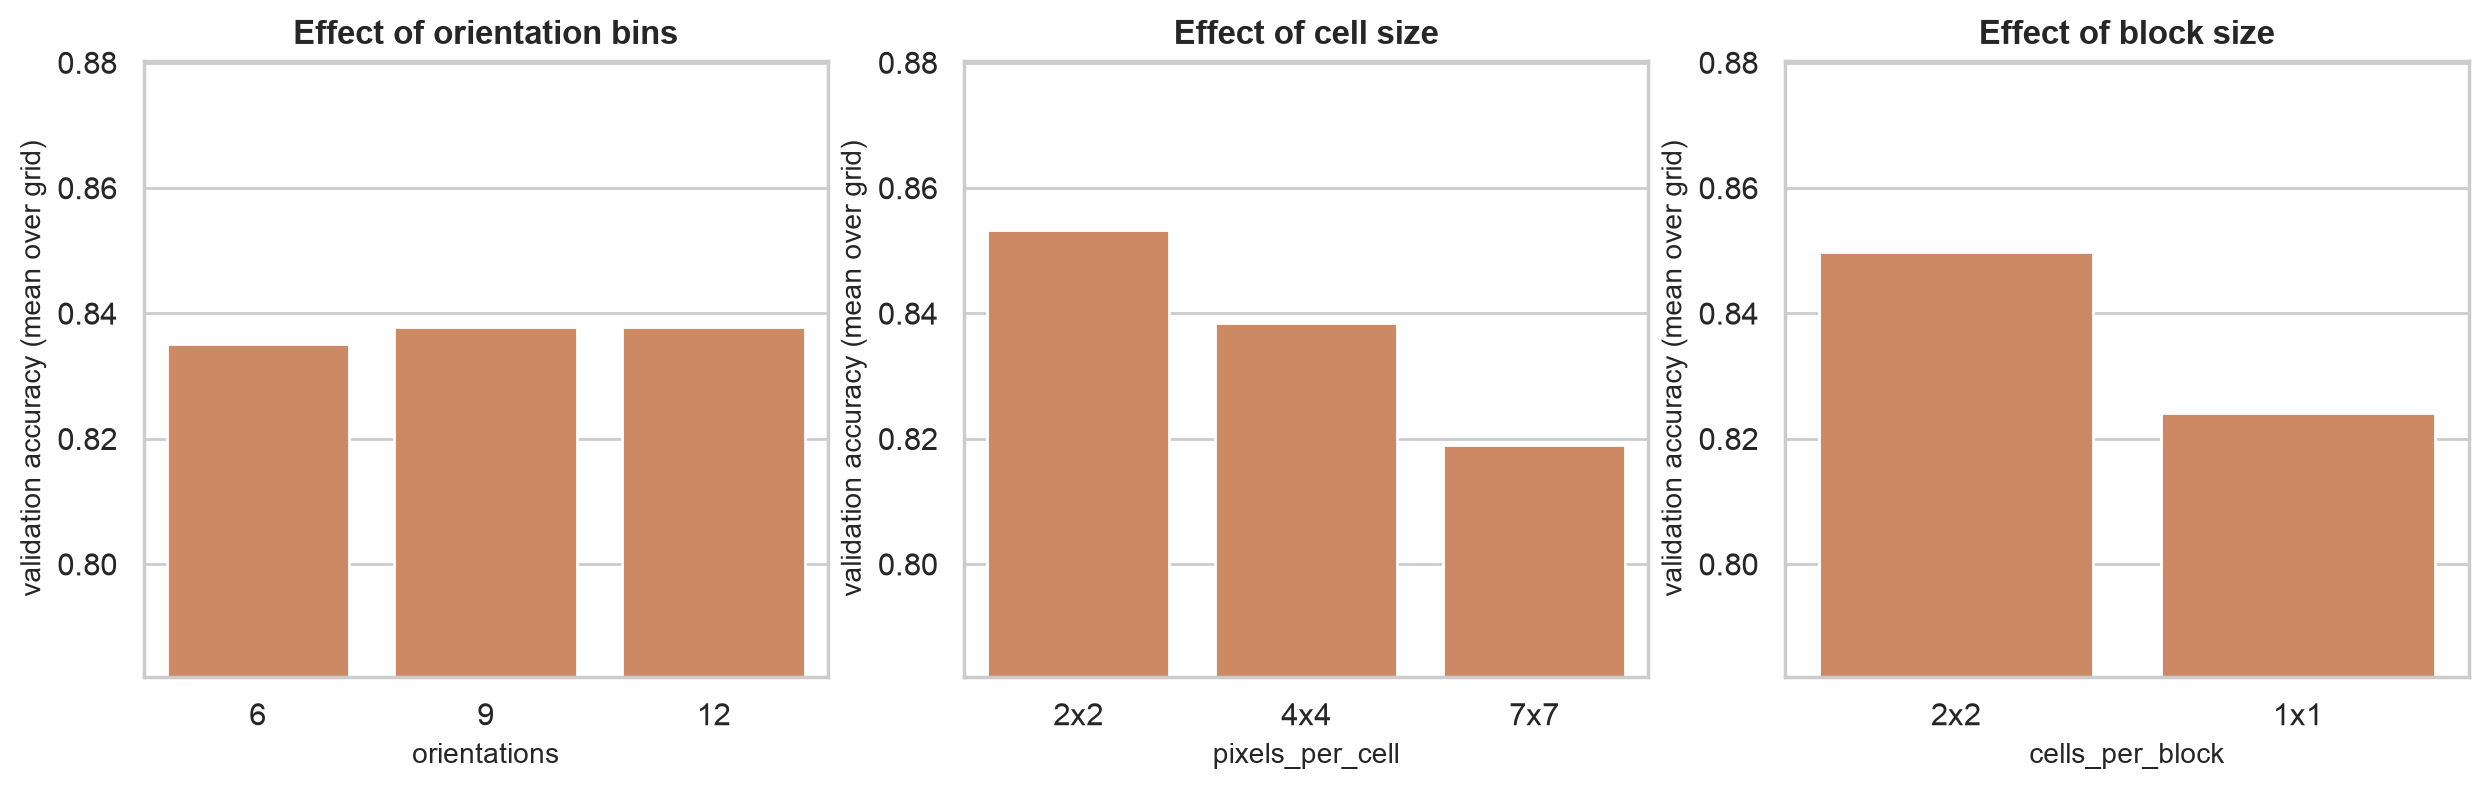
\includegraphics[width=\textwidth]{fe_01_hog_ablation.png}\caption{HOG hyper-parameter ablation (validation accuracy).}\label{fig:hogab}\end{figure*}

\subsection{Shape statistics (16-d)}
\texttt{shape\_stats} computes interpretable global descriptors: mean and standard deviation of intensity, ink fraction (pixels $>0.1$), bounding-box height, width and aspect ratio, centroid row/column, left--right and top--bottom symmetry ($1-\|I-\mathrm{flip}(I)\|_1/(2\|I\|_1)$), Sobel edge density (\texttt{scipy.ndimage.sobel}), top/bottom-half ink mass, width of the top and bottom rows, and the gap between legs. Each is divided by a fixed constant to bring it to roughly $[0,1]$ so that it does not dominate the HOG block in distance/kernel models. Fig.~\ref{fig:stats} shows the class profile; a Random Forest ranks ink fraction, aspect ratio and bottom width highest. Concatenated with HOG they form the \texttt{hog\_stats} set (880-d).

\begin{figure}[t]\centering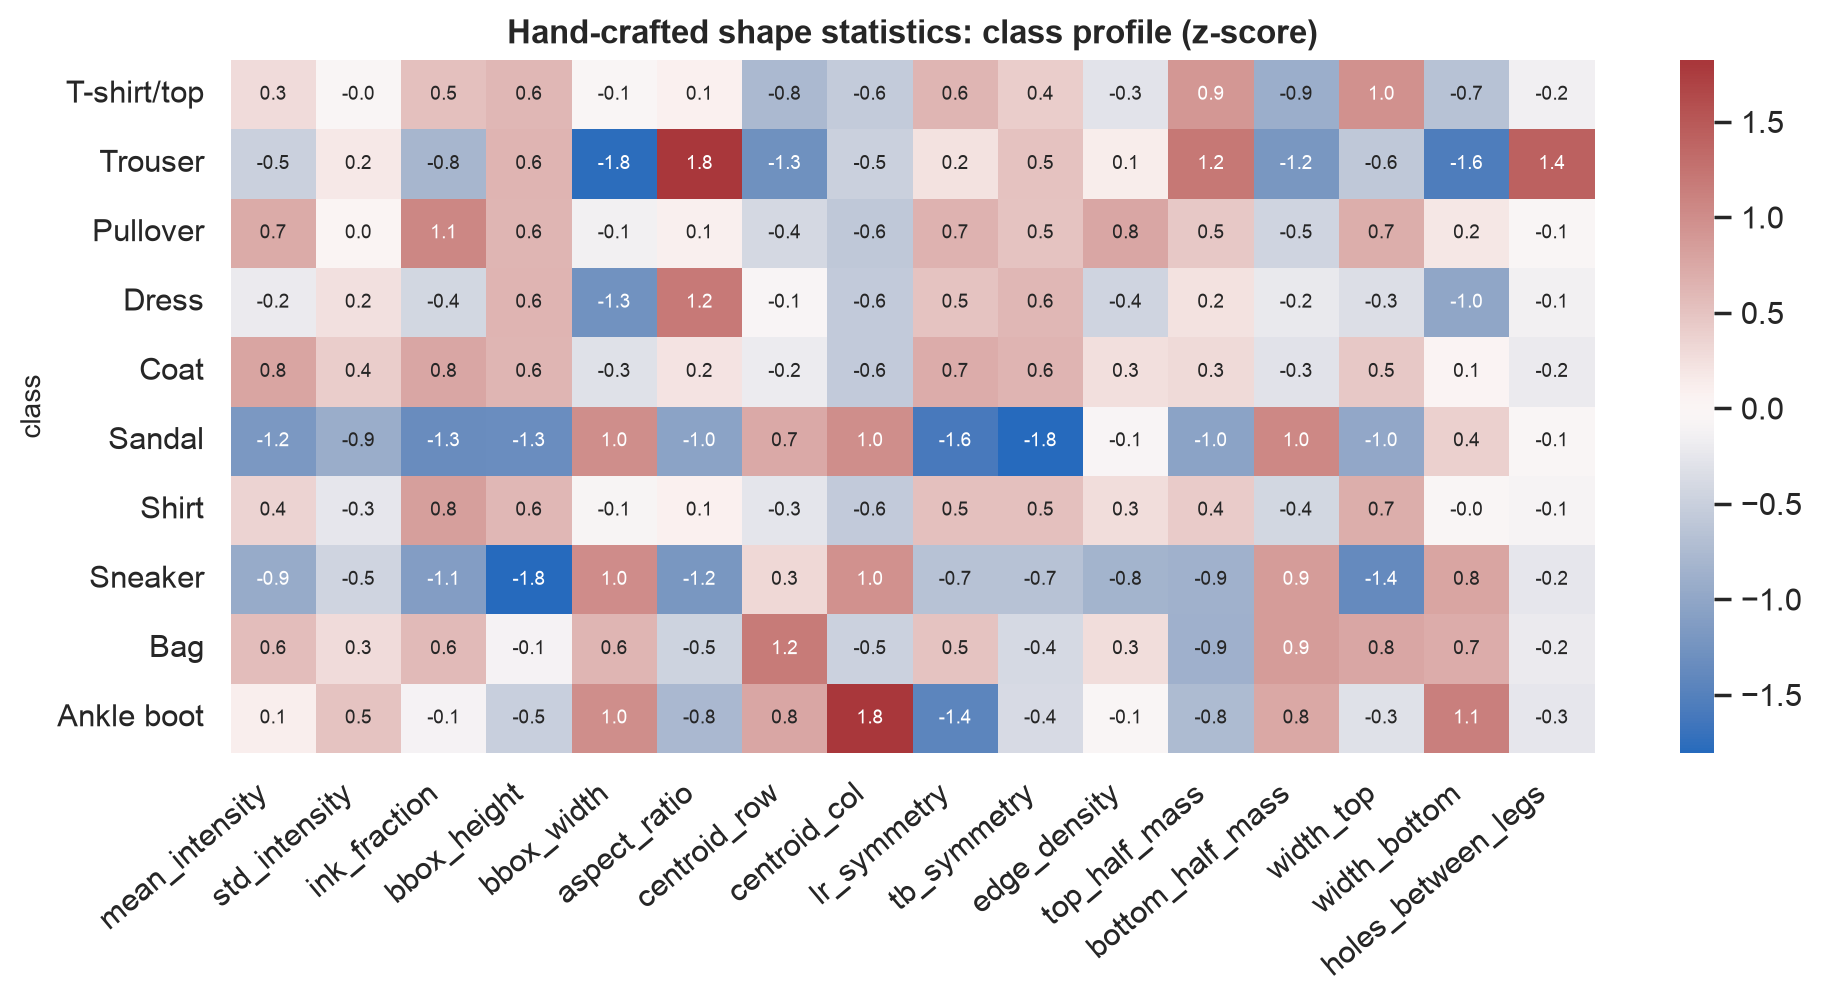
\includegraphics[width=\columnwidth]{fe_03_shape_stats_profile.png}\caption{Class profile of the 16 shape statistics (z-score).}\label{fig:stats}\end{figure}

\subsection{PCA reference and probe comparison}
PCA (\texttt{sklearn.decomposition.PCA}) with 100--200 components gives 0.857--0.862 probe accuracy, equal to using all 784 pixels (0.855), confirming redundancy but also showing that a linear projection cannot add new information (Fig.~\ref{fig:pcasweep}). Under the same probe, pixels reach 0.855, HOG 0.884 and HOG+stats 0.889 (validation).

\begin{figure}[t]\centering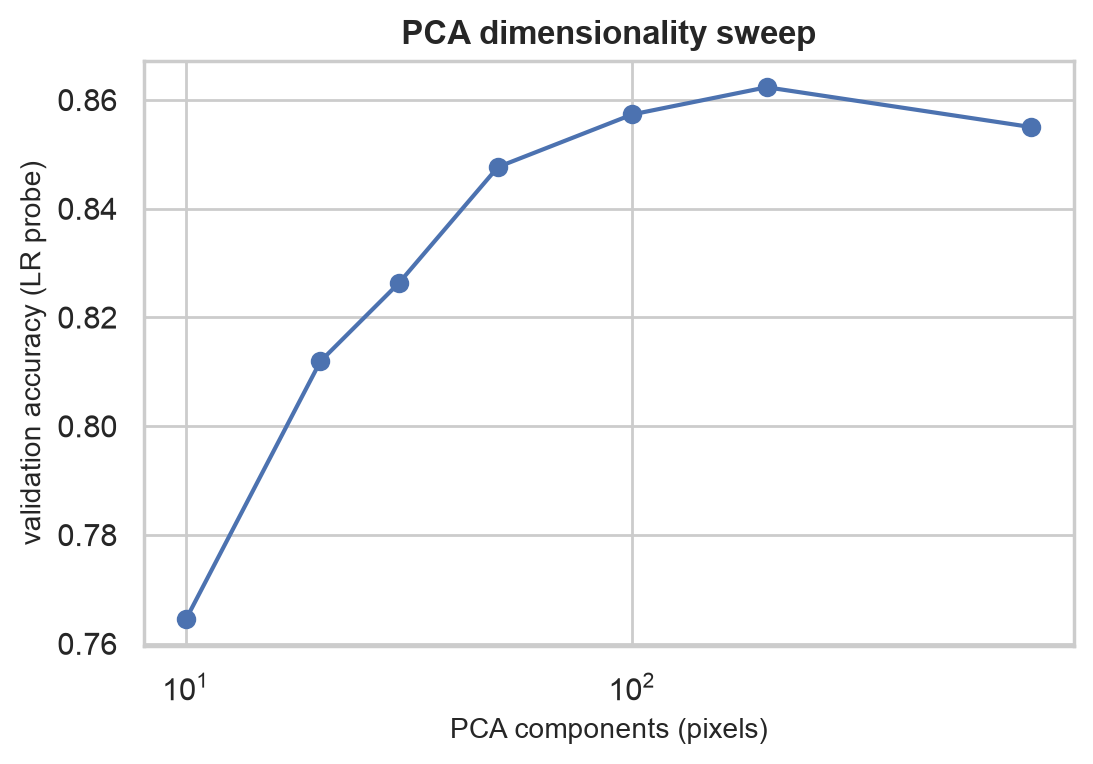
\includegraphics[width=0.85\columnwidth]{fe_05_pca_sweep.png}\caption{PCA dimension sweep (LR probe).}\label{fig:pcasweep}\end{figure}

%=====================================================================
\section{Methodology: Models and Theory}\label{sec:method}
All models are from \texttt{scikit-learn}~\cite{pedregosa2011}; \texttt{scikit-image}~\cite{vanderwalt2014} provides HOG.

\textbf{Logistic Regression} (multinomial, \texttt{LogisticRegression}, L-BFGS, max 300 iterations). It minimises $-\sum_i\log\mathrm{softmax}(Wx_i+b)_{y_i}+\frac{1}{2C}\|W\|_2^2$. Inputs are standardised (\texttt{StandardScaler} inside a \texttt{Pipeline}, fitted on the training data only). Parameters: $10\cdot d+10$.

\textbf{$k$-Nearest Neighbours} (\texttt{KNeighborsClassifier}). Predicts the (distance-weighted) majority label of the $k$ closest training images in Euclidean distance. Non-parametric: the stored matrix is the model.

\textbf{Random Forest} (\texttt{RandomForestClassifier}, 300 trees, $\sqrt d$ candidate features per split). Bootstrap-aggregated decision trees that each split on a pixel/feature threshold minimising Gini impurity; prediction is the average class vote.

\textbf{SVM with RBF kernel} (\texttt{SVC}). Solves the soft-margin dual with kernel $K(x,x')=\exp(-\gamma\|x-x'\|^2)$, $\gamma=1/(d\,\mathrm{Var}(X))$ (\texttt{gamma='scale'}), one-vs-one for 10 classes. $C$ controls the margin/error trade-off.

\textbf{Why HOG may help differently.} A linear model on pixels can only weigh each pixel independently, so any neighbourhood interaction (an edge) has to be created by the descriptor. A kernel SVM or a forest can construct such interactions itself, so we expect the benefit of HOG to shrink with model flexibility. This hypothesis is tested below.

\textbf{Metrics.} Accuracy; macro-F1 $=\frac1{10}\sum_c F1_c$; per-class recall $R_c=TP_c/(TP_c+FN_c)$; parameter count (definition per family, Table~\ref{tab:params}); inference time per image (single-threaded \texttt{predict} on the 10{,}000 test images) plus feature-extraction time.

\begin{table}[t]\centering\caption{Definition of ``parameters''.}\label{tab:params}
\begin{tabular}{@{}ll@{}}\toprule Model & Counted numbers\\\midrule
LogReg & weights + biases\\
kNN & stored training matrix\\
Random Forest & 2 per internal node (feature, threshold)\\
SVM-RBF & support vectors + dual coefficients + intercepts\\\bottomrule\end{tabular}\end{table}

%=====================================================================
\section{Experimental Protocol}
\begin{enumerate}
\item \textbf{Split.} The official 60{,}000/10{,}000 split is untouched. A stratified 20\% of the training set (12{,}000 images, \texttt{train\_test\_split}, seed 42) forms the validation set; 48{,}000 images remain for fitting.
\item \textbf{Tuning.} Each model's small grid (Table~\ref{tab:grid}) is scored on validation accuracy. The SVM grid is fitted on a stratified 15{,}000-image subsample of the 48{,}000 because of its cubic worst-case cost, but scored on the full validation set.
\item \textbf{Final fit.} The chosen configuration is refit on train+validation (60{,}000 images) and evaluated once on the test set.
\item \textbf{Fairness.} Identical seed, scaling policy and tuning budget for all feature sets; the validation set never contains test images; features such as the scaler are fitted on training data only.
\end{enumerate}

\begin{table}[t]\centering\caption{Hyper-parameter grids.}\label{tab:grid}
\begin{tabular}{@{}ll@{}}\toprule Model & Grid\\\midrule
LogReg & $C\in\{0.001,0.01,0.1,1\}$\\
kNN & $k\in\{3,5,9\}$, weights $\in\{$uniform, distance$\}$\\
RF & depth $\in\{20,\text{None}\}$, min leaf $\in\{1,2\}$, 300 trees\\
SVM-RBF & $C\in\{1,5,20\}$, $\gamma=$ `scale'\\\bottomrule\end{tabular}\end{table}

%=====================================================================
\section{Results}\label{sec:results}
Table~\ref{tab:main} gives the test results; Fig.~\ref{fig:overview} visualises them.

\begin{table*}[t]\centering\caption{Test-set results (10{,}000 images). Latency is \texttt{predict} time per image, single thread; HOG extraction adds 0.14 ms (HOG) or 0.19 ms (HOG+stats) per image.}\label{tab:main}
\begin{tabular}{@{}llrrrrrrr@{}}\toprule
Model & Features & Val acc & Test acc & Macro-F1 & Fit (s) & Infer (ms) & Parameters\\\midrule
LogReg & pixels & 0.8633 & 0.8456 & 0.8447 & 8.8 & 0.0013 & 7{,}850\\
LogReg & HOG & 0.8913 & 0.8852 & 0.8848 & 6.1 & 0.0014 & 8{,}650\\
LogReg & HOG+stats & 0.8963 & 0.8894 & 0.8890 & 7.8 & 0.0013 & 8{,}810\\\midrule
kNN & pixels & 0.8592 & 0.8561 & 0.8564 & 0.1 & 0.316 & 47.0M\\
kNN & HOG & 0.8821 & 0.8774 & 0.8777 & 0.0 & 0.271 & 51.8M\\
kNN & HOG+stats & 0.8826 & 0.8776 & 0.8780 & 0.0 & 0.313 & 52.8M\\\midrule
RF & pixels & 0.8862 & 0.8760 & 0.8746 & 22.8 & 0.037 & 2.54M\\
RF & HOG & 0.8823 & 0.8781 & 0.8769 & 39.5 & 0.042 & 3.23M\\
RF & HOG+stats & 0.8848 & 0.8821 & 0.8811 & 41.3 & 0.041 & 2.51M\\\midrule
SVM-RBF & pixels & 0.8888 & 0.8988 & 0.8985 & 192 & 4.53 & 15.0M\\
SVM-RBF & HOG & 0.8990 & \textbf{0.9130} & \textbf{0.9130} & 207 & 5.36 & 18.1M\\
SVM-RBF & HOG+stats & 0.9008 & \textbf{0.9137} & \textbf{0.9137} & 223 & 5.28 & 17.5M\\\bottomrule
\end{tabular}\end{table*}

\begin{figure*}[t]\centering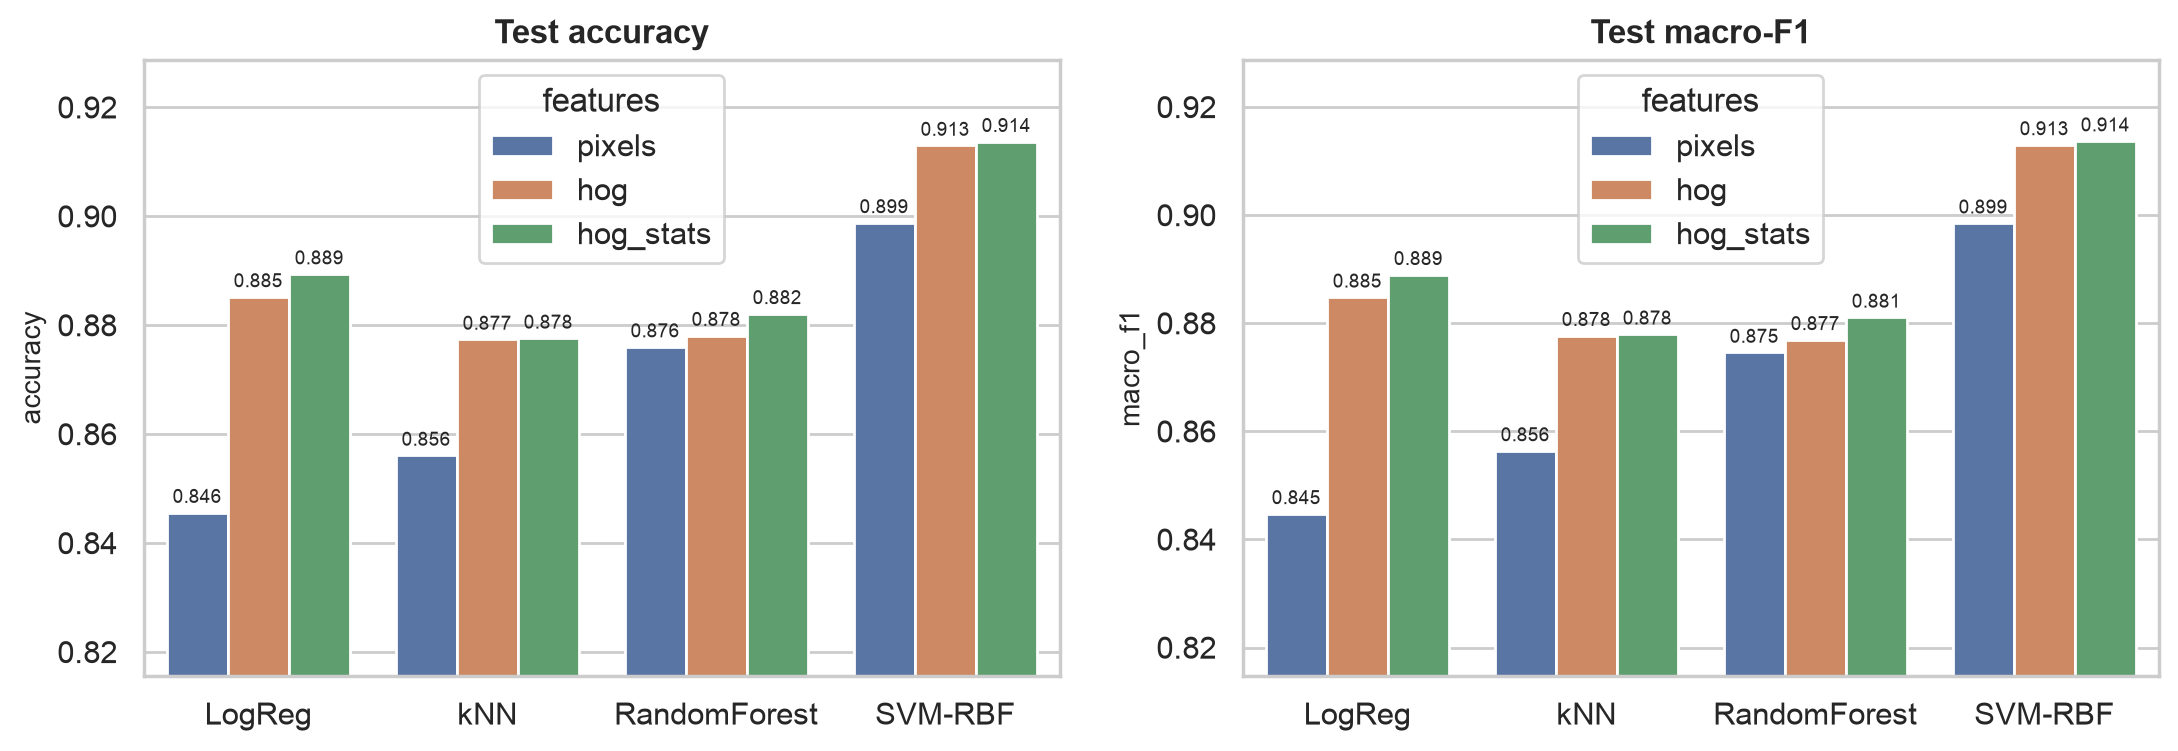
\includegraphics[width=\textwidth]{res_01_accuracy_f1_overview.png}\caption{Test accuracy and macro-F1 for all configurations.}\label{fig:overview}\end{figure*}

\textbf{Does HOG help?} Table~\ref{tab:mc} reports paired McNemar tests (continuity-corrected $\chi^2$, 1 d.o.f.) between pixels and HOG for each learner. HOG improves Logistic Regression (+3.96 points), $k$-NN (+2.13) and SVM (+1.42) significantly, while Random Forest is statistically unchanged (+0.21, $p=0.49$). This supports the hypothesis that the benefit shrinks with model flexibility, and the Random Forest, which can threshold single pixels hierarchically, gains nothing. The 95\% bootstrap intervals (1{,}000 resamples) for the best model are [0.908, 0.919] (HOG+stats) and [0.907, 0.919] (HOG), clearly above the best pixel model [0.893, 0.905].

\begin{table}[t]\centering\caption{McNemar test, pixels vs.\ HOG.}\label{tab:mc}
\begin{tabular}{@{}lrrrrr@{}}\toprule Model & $\Delta$acc & only-pix & only-HOG & $\chi^2$ & $p$\\\midrule
LogReg & +0.0396 & 411 & 807 & 128.1 & $<10^{-6}$\\
kNN & +0.0213 & 515 & 728 & 36.2 & $2\!\times\!10^{-9}$\\
RF & +0.0021 & 404 & 425 & 0.48 & 0.49\\
SVM & +0.0142 & 345 & 487 & 23.9 & $10^{-6}$\\\bottomrule\end{tabular}\end{table}

\textbf{HOG+stats.} Adding the 16 statistics helps Logistic Regression (+0.4) and Random Forest (+0.4) but is neutral for kNN and SVM (+0.07); gains are within bootstrap noise, so we regard HOG alone as the default. Before normalising the statistics to $[0,1]$, the SVM on HOG+stats scored only 0.8868, showing that unscaled heterogeneous features can dominate a kernel's distance.

\textbf{Data efficiency.} With a fixed Logistic Regression (Fig.~\ref{fig:lc}), HOG is better at every size, and at 5{,}000 images it already matches pixels at 20{,}000 (0.863 vs.\ 0.858).

\textbf{Cost.} Fig.~\ref{fig:pareto} shows accuracy against latency. Logistic Regression is $\sim$4{,}000$\times$ faster than the SVM at inference and 2{,}000$\times$ smaller, at a cost of 2.8 points. kNN stores 47--53 million numbers. The Random Forest is a good middle option at 0.04 ms but gains nothing from HOG.

\begin{figure}[t]\centering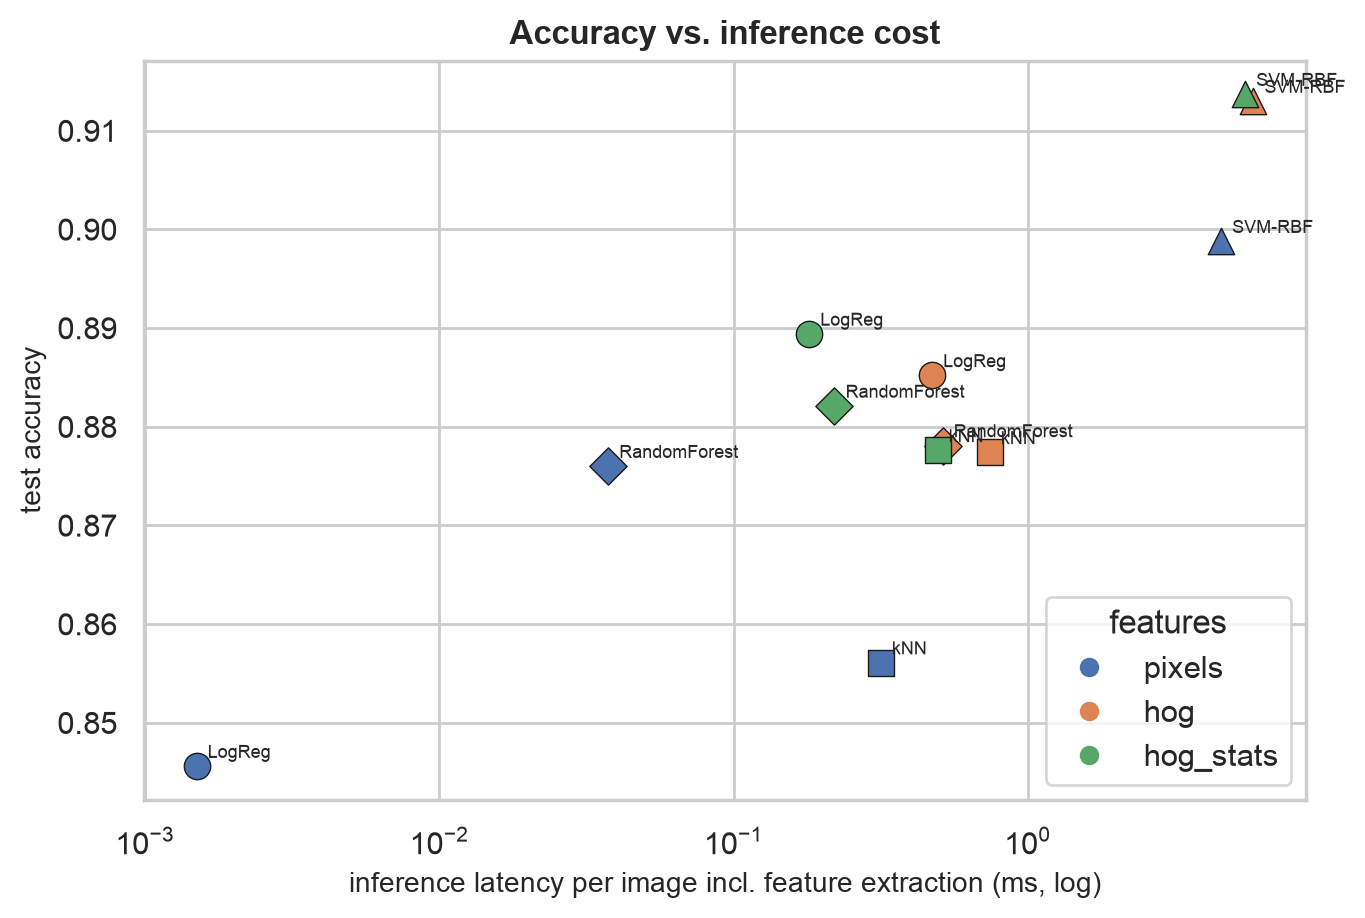
\includegraphics[width=\columnwidth]{res_07_accuracy_vs_latency.png}\caption{Accuracy versus inference latency.}\label{fig:pareto}\end{figure}
\begin{figure}[t]\centering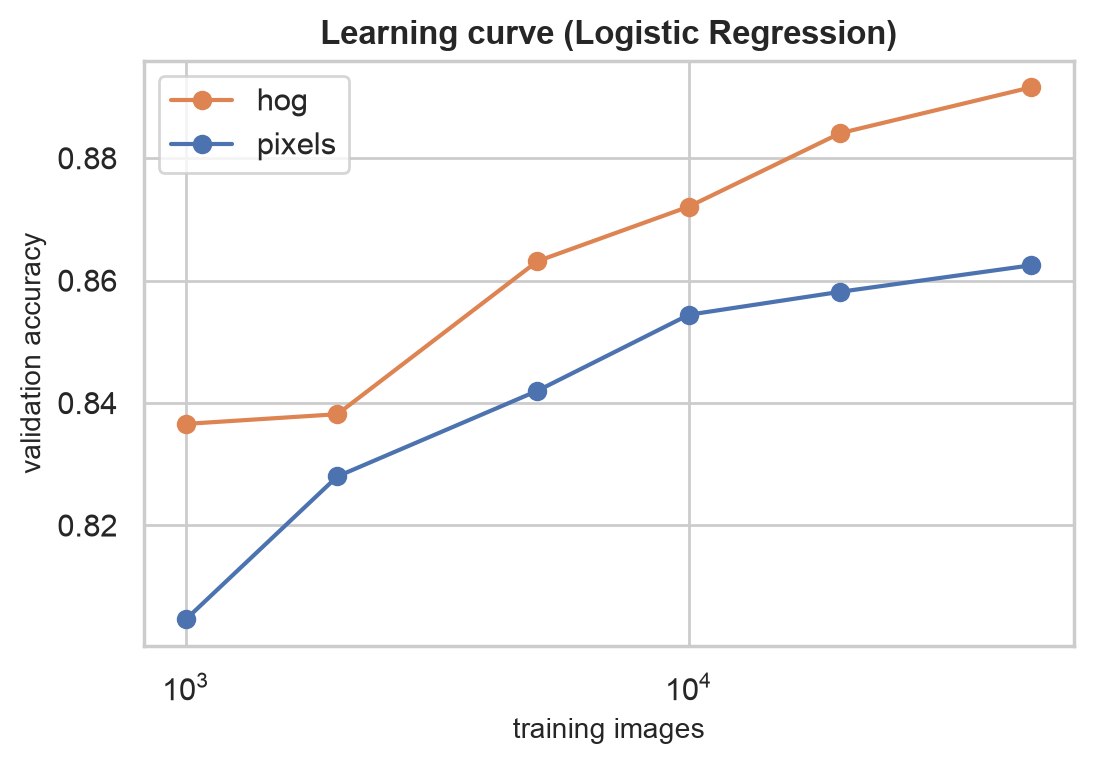
\includegraphics[width=0.85\columnwidth]{res_08_learning_curve.png}\caption{Learning curves (Logistic Regression).}\label{fig:lc}\end{figure}

\textbf{Per-class recall.} Table~\ref{tab:recall} lists the best pixel and best HOG models. Trouser, Bag, Sandal, Sneaker and Ankle boot exceed 0.96 recall for both, while Shirt (0.705 $\to$ 0.750), Pullover (0.830 $\to$ 0.856), Coat (0.838 $\to$ 0.875) and T-shirt (0.862 $\to$ 0.873) are the weak classes; HOG helps these most.

\begin{table}[t]\centering\caption{Per-class recall of SVM-RBF.}\label{tab:recall}
\begin{tabular}{@{}lrr@{}}\toprule Class & Pixels & HOG\\\midrule
T-shirt/top & 0.862 & 0.873\\ Trouser & 0.970 & 0.975\\ Pullover & 0.830 & 0.856\\ Dress & 0.911 & 0.918\\ Coat & 0.838 & 0.875\\
Sandal & 0.968 & 0.971\\ Shirt & 0.705 & 0.750\\ Sneaker & 0.966 & 0.967\\ Bag & 0.979 & 0.981\\ Ankle boot & 0.959 & 0.964\\\bottomrule\end{tabular}\end{table}

\begin{figure*}[t]\centering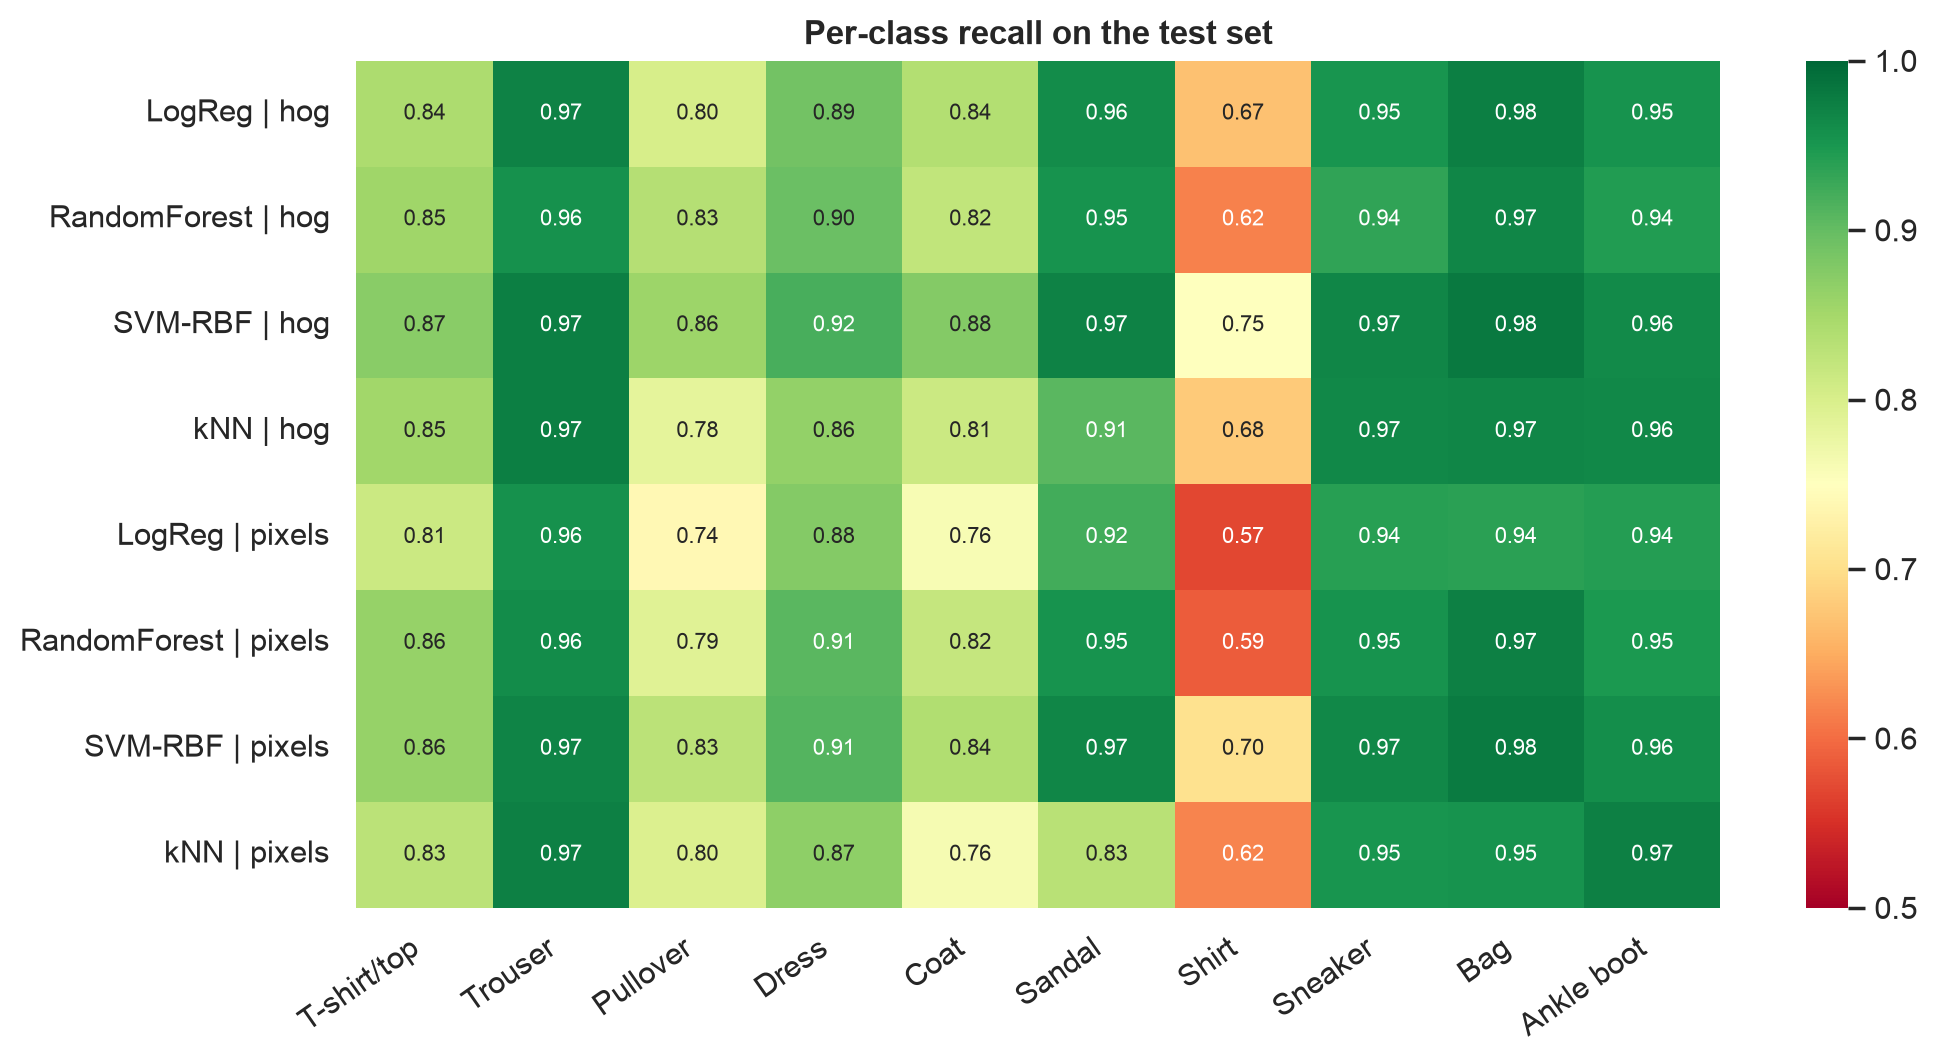
\includegraphics[width=\textwidth]{res_02_per_class_recall.png}\caption{Per-class test recall for all models (pixels and HOG).}\label{fig:recallhm}\end{figure*}

%=====================================================================
\section{Error Analysis}\label{sec:errors}
Fig.~\ref{fig:cm} shows the confusion matrices of the best pixel and the best HOG model (both SVM-RBF), and Fig.~\ref{fig:cmdiff} their difference. The largest confusions for the pixel model are Shirt$\to$T-shirt (120), T-shirt$\to$Shirt (91), Shirt$\to$Pullover (83), Coat$\to$Pullover (79) and Pullover$\to$Coat (77), exactly the pairs predicted by the mean-image distances in Section~\ref{sec:eda}.

The share of all errors that fall inside the upper-body group (T-shirt, Pullover, Coat, Shirt) is 58--65\% for every model: 64.8\% (SVM pixels, 656 of 1{,}012 errors) and 63.4\% (SVM HOG, 552 of 870). HOG removes 142 errors in total, 104 of them in this group, but it cannot remove the ambiguity because at $28\times28$ the discriminating details of a shirt (collar, buttons, cuffs) are one or two pixels wide. Fig.~\ref{fig:mis} shows misclassified examples: several are ambiguous even for a human.

\begin{figure*}[t]\centering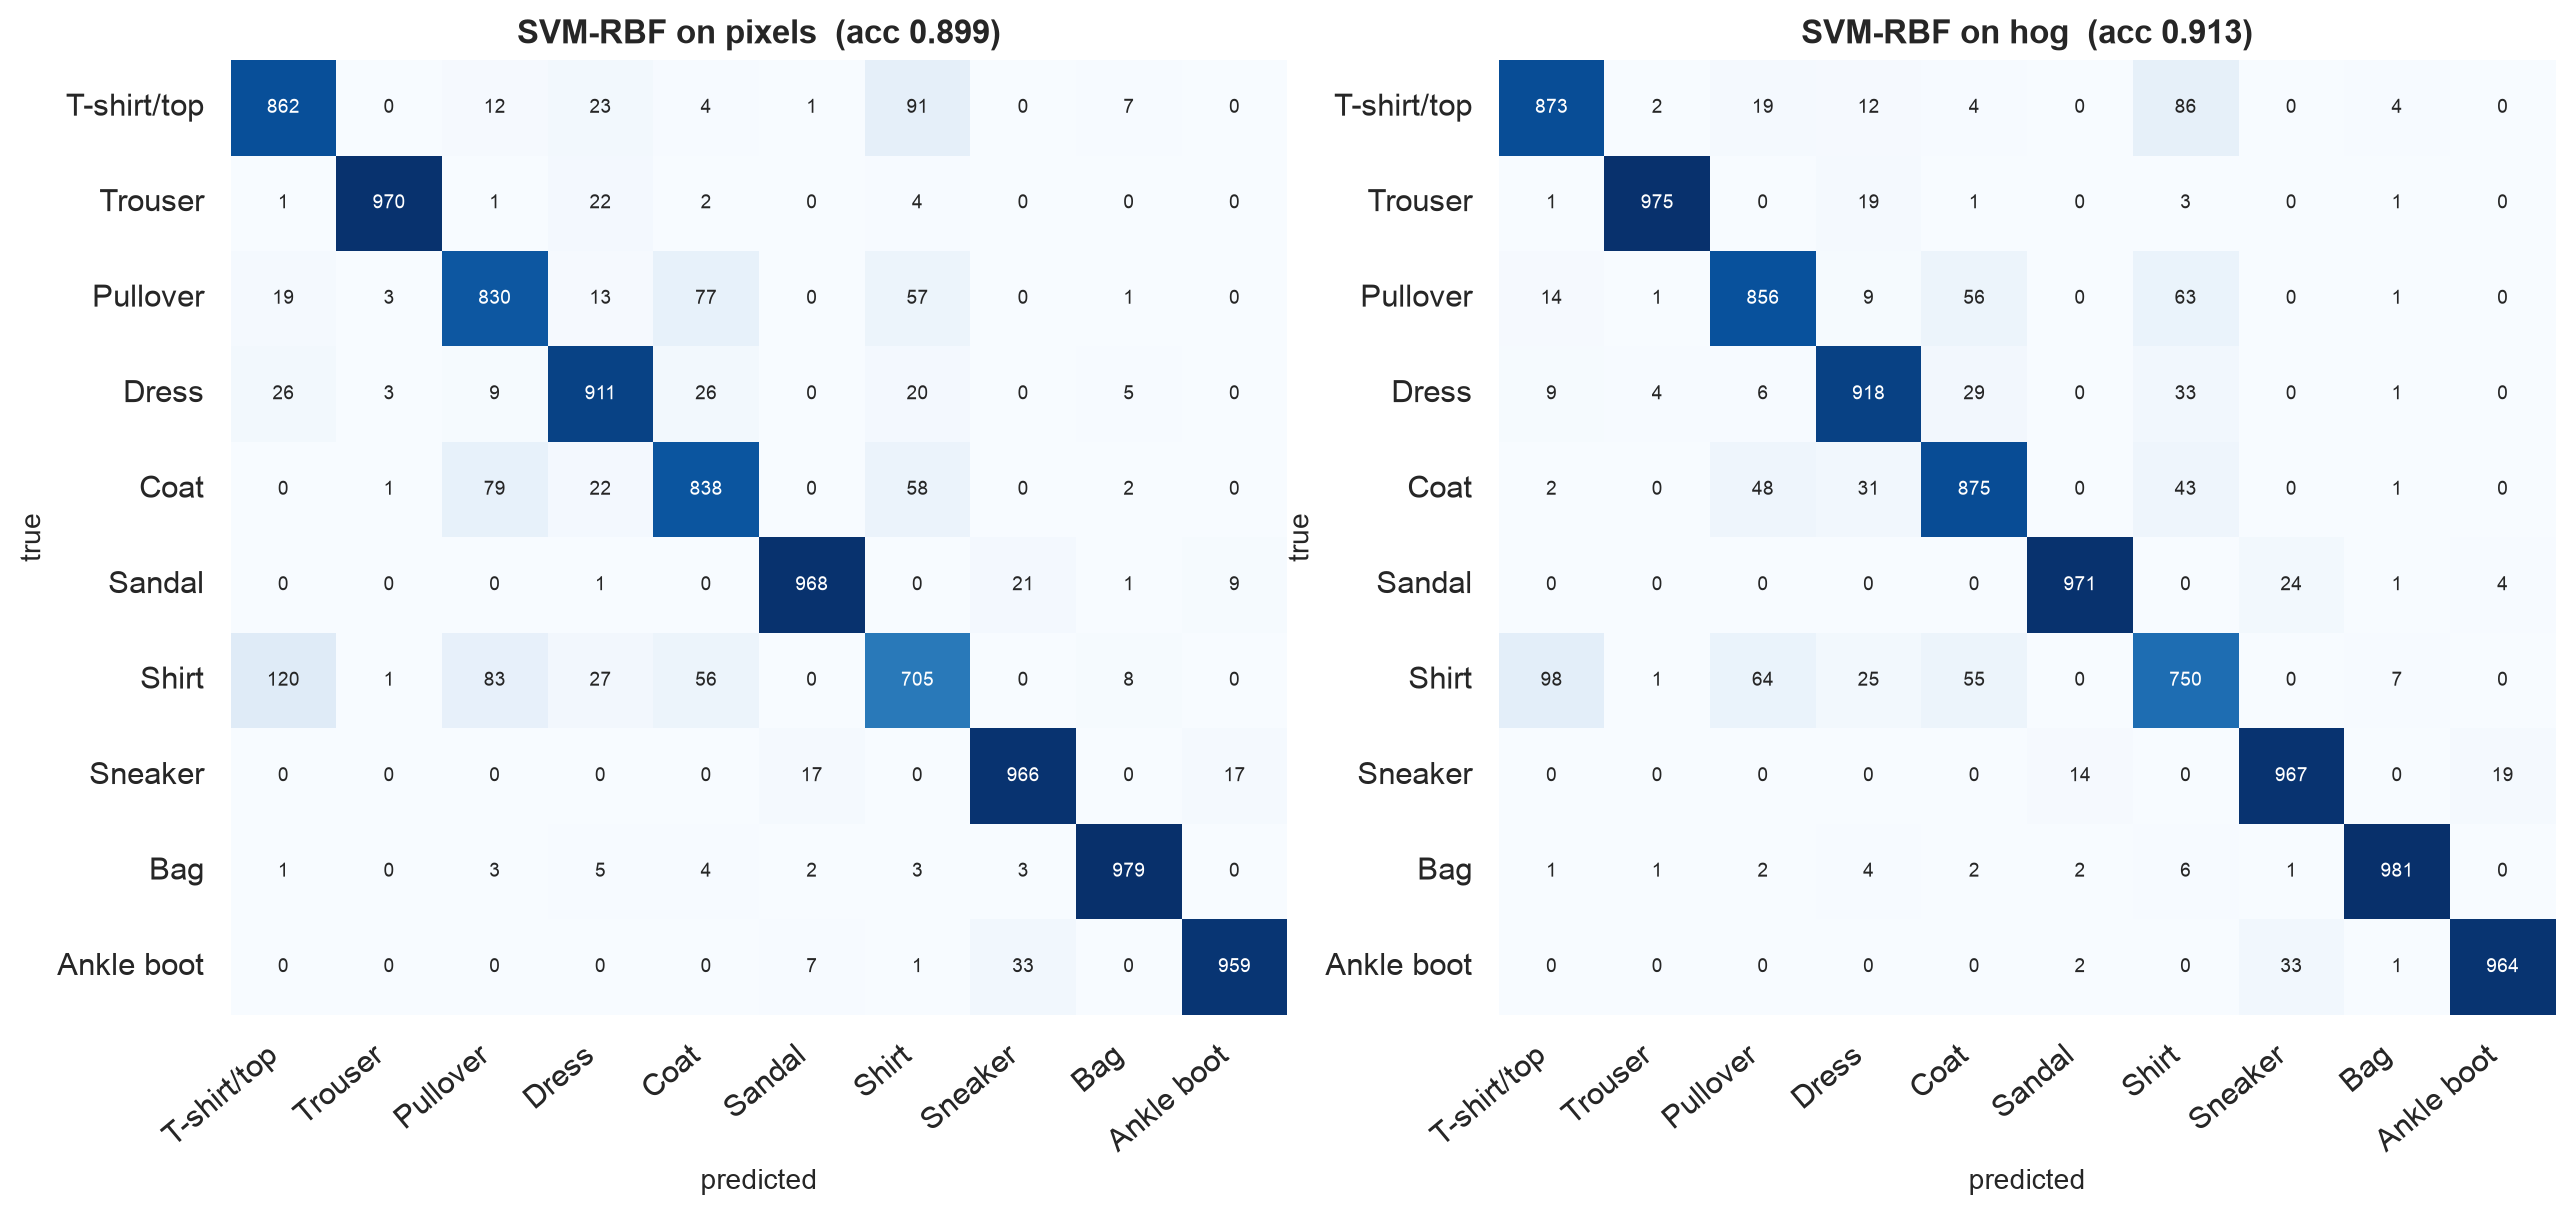
\includegraphics[width=\textwidth]{res_03_confusion_best_pixels_vs_best_hog.png}\caption{Confusion matrices: best pixel model vs.\ best HOG model.}\label{fig:cm}\end{figure*}
\begin{figure}[t]\centering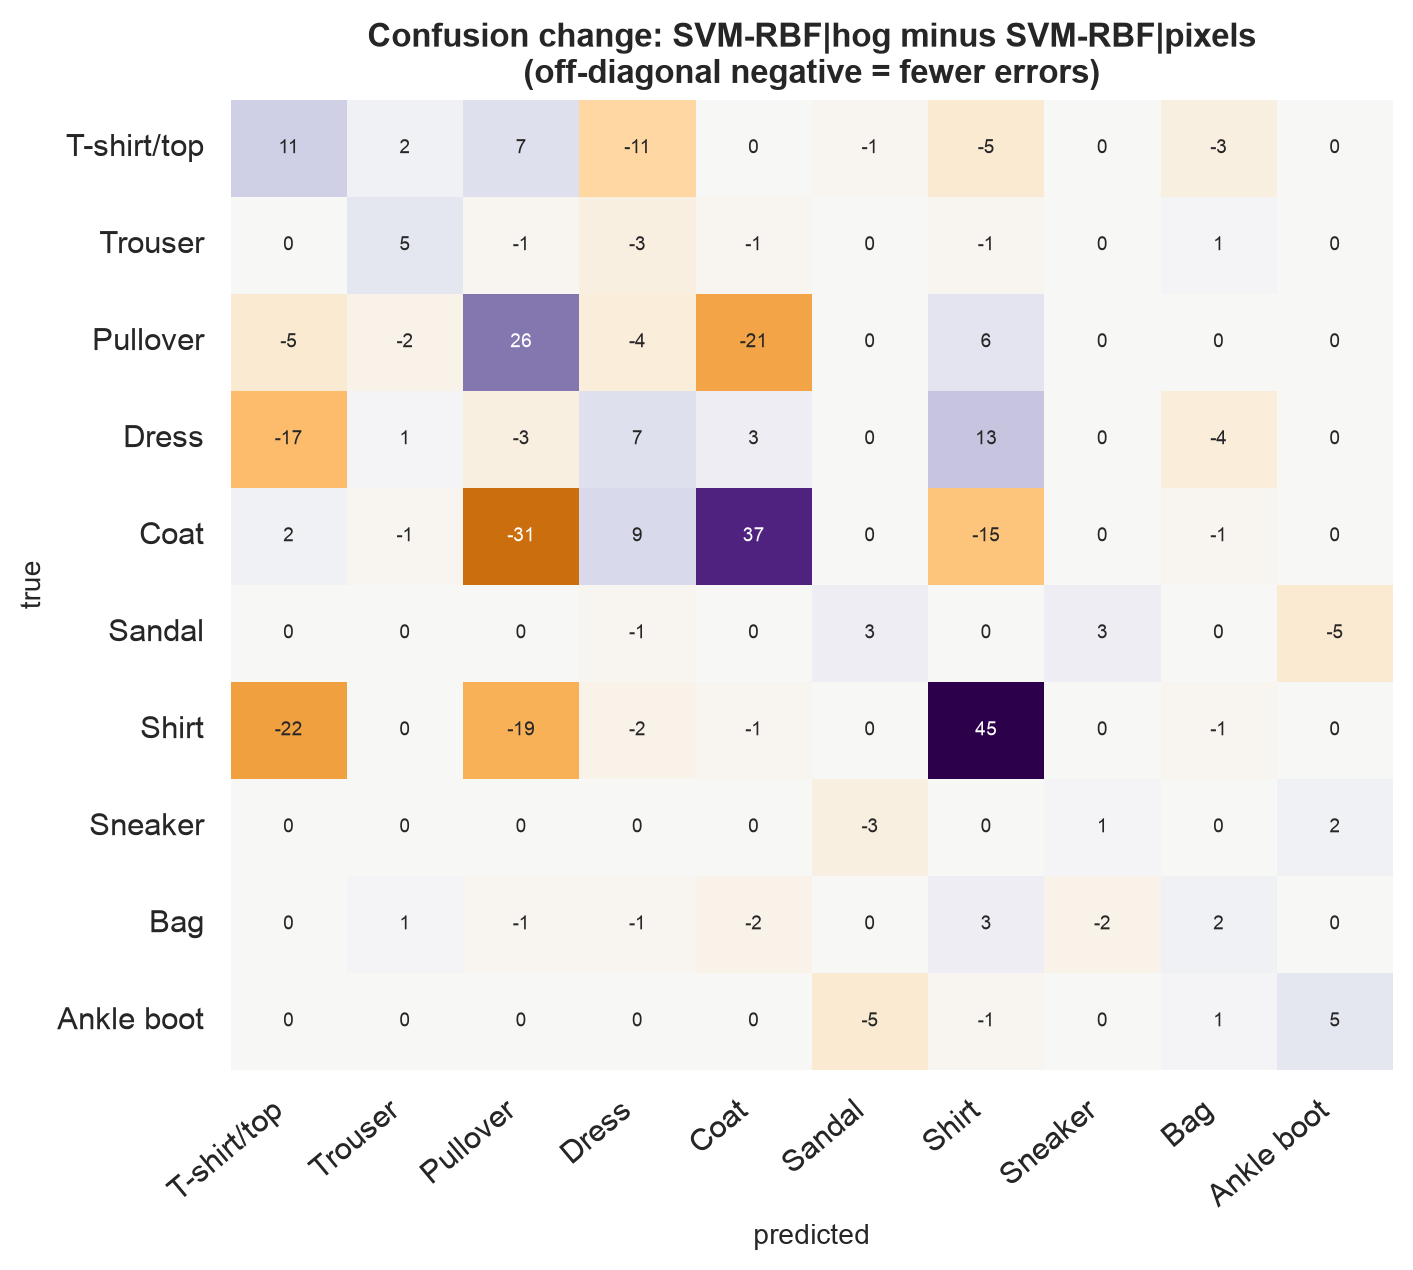
\includegraphics[width=0.9\columnwidth]{res_04_confusion_difference.png}\caption{Confusion change (HOG minus pixels).}\label{fig:cmdiff}\end{figure}
\begin{figure}[t]\centering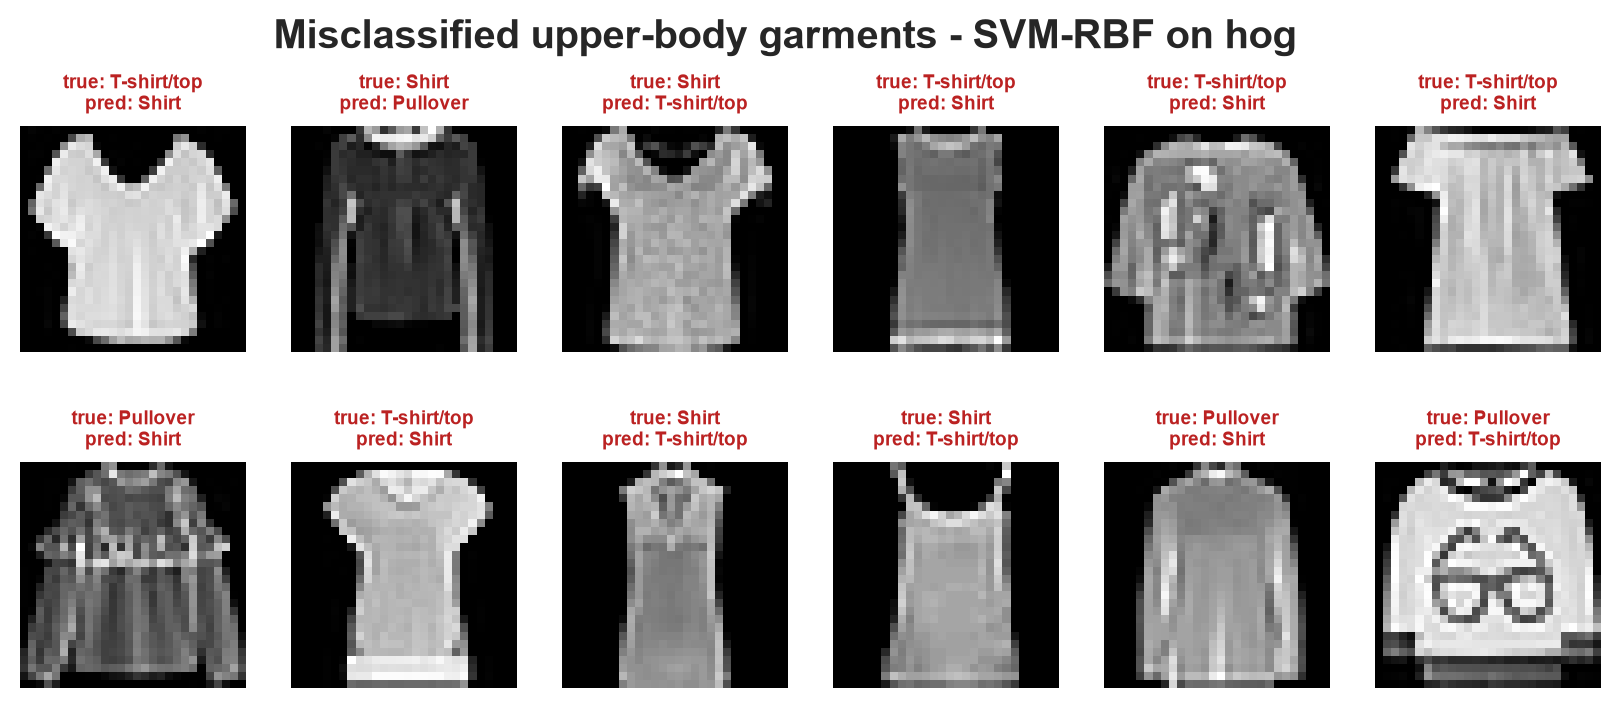
\includegraphics[width=\columnwidth]{res_06b_misclassified_best_hog.png}\caption{Misclassified upper-body garments (SVM, HOG).}\label{fig:mis}\end{figure}

%=====================================================================
\section{Discussion, Limitations and Phase~2}
\textbf{Answer to the research question.} A fixed HOG descriptor is a cheap (0.14 ms) and statistically significant improvement for linear, instance-based and kernel learners, and the best classical model is a kernel SVM on HOG (91.3\%). It does not help a Random Forest. Flattened pixels are not always worse; they are worse when the learner cannot build neighbourhood interactions itself.

\textbf{Limitations.} (i) The HOG configuration was selected with a Logistic-Regression probe, not per classifier. (ii) A single validation split is used; test uncertainty is bootstrap-based but there is no repeated cross-validation. (iii) The SVM is tuned on a 15{,}000-image subsample. (iv) Grids are small. (v) The $28\times28$ grayscale resolution discards the texture that separates shirts from T-shirts.

\textbf{Phase~2.} A two- or three-block CNN with pooling, dropout and early stopping will be trained on the \emph{same} splits and compared on the same metrics. The CNN can learn its own hierarchical filters and may resolve the upper-body group better than any fixed descriptor.

%=====================================================================
\section{Conclusion}
We built a reproducible Phase-1 pipeline for Fashion-MNIST: audit and EDA, three feature sets, four classifiers, strict validation, paired significance tests and error analysis. HOG improves three of four classifiers significantly; the best model reaches 91.3\% accuracy and 0.913 macro-F1; and the Shirt/T-shirt/Pullover/Coat group dominates the remaining errors.

\section*{Reproducibility and Code}
All code, notebooks, the Streamlit presentation and raw result tables are in the project repository (\texttt{README.md}). Seeds are fixed (42); \texttt{scripts/run\_all.sh} regenerates every figure and table.

\appendices
\section{Software Components}
\begin{table}[h]\centering\caption{Main functions used.}
\begin{tabular}{@{}p{0.34\columnwidth}p{0.58\columnwidth}@{}}\toprule
Function / class & Purpose\\\midrule
\texttt{gzip}, \texttt{np.frombuffer} & read IDX files\\
\texttt{train\_test\_split} (stratify) & validation split from train\\
\texttt{skimage.feature.hog} & HOG descriptor\\
\texttt{scipy.ndimage.sobel} & edge density\\
\texttt{PCA}, \texttt{TSNE} & dimensionality reduction/visualisation\\
\texttt{f\_classif} & pixel F-score\\
\texttt{StandardScaler}, \texttt{Pipeline} & scaling inside the model\\
\texttt{LogisticRegression}, \texttt{KNeighborsClassifier}, \texttt{RandomForestClassifier}, \texttt{SVC} & the four learners\\
\texttt{accuracy\_score}, \texttt{f1\_score}, \texttt{recall\_score}, \texttt{confusion\_matrix} & metrics\\
\texttt{scipy.stats.ks\_2samp}, \texttt{chi2} & KS test, McNemar test\\
\texttt{joblib} & parallel feature extraction, model saving\\
\texttt{matplotlib}, \texttt{seaborn}, \texttt{plotly}, \texttt{streamlit} & figures and presentation app\\\bottomrule
\end{tabular}\end{table}

\begin{thebibliography}{99}
\bibitem{xiao2017} H.~Xiao, K.~Rasul, and R.~Vollgraf, ``Fashion-MNIST: a novel image dataset for benchmarking machine learning algorithms,'' arXiv:1708.07747, 2017.
\bibitem{lecun1998} Y.~LeCun, L.~Bottou, Y.~Bengio, and P.~Haffner, ``Gradient-based learning applied to document recognition,'' \emph{Proc. IEEE}, vol.~86, no.~11, pp.~2278--2324, 1998.
\bibitem{dalal2005} N.~Dalal and B.~Triggs, ``Histograms of oriented gradients for human detection,'' in \emph{Proc. IEEE CVPR}, 2005, pp.~886--893.
\bibitem{lowe2004} D.~G. Lowe, ``Distinctive image features from scale-invariant keypoints,'' \emph{Int. J. Comput. Vis.}, vol.~60, no.~2, pp.~91--110, 2004.
\bibitem{ojala2002} T.~Ojala, M.~Pietik\"ainen, and T.~M\"aenp\"a\"a, ``Multiresolution gray-scale and rotation invariant texture classification with local binary patterns,'' \emph{IEEE TPAMI}, vol.~24, no.~7, pp.~971--987, 2002.
\bibitem{hastie2009} T.~Hastie, R.~Tibshirani, and J.~Friedman, \emph{The Elements of Statistical Learning}, 2nd ed. Springer, 2009.
\bibitem{cover1967} T.~Cover and P.~Hart, ``Nearest neighbor pattern classification,'' \emph{IEEE Trans. Inf. Theory}, vol.~13, no.~1, pp.~21--27, 1967.
\bibitem{breiman2001} L.~Breiman, ``Random forests,'' \emph{Machine Learning}, vol.~45, no.~1, pp.~5--32, 2001.
\bibitem{cortes1995} C.~Cortes and V.~Vapnik, ``Support-vector networks,'' \emph{Machine Learning}, vol.~20, no.~3, pp.~273--297, 1995.
\bibitem{jolliffe2002} I.~T. Jolliffe, \emph{Principal Component Analysis}, 2nd ed. Springer, 2002.
\bibitem{vandermaaten2008} L.~van~der Maaten and G.~Hinton, ``Visualizing data using t-SNE,'' \emph{J. Mach. Learn. Res.}, vol.~9, pp.~2579--2605, 2008.
\bibitem{mcnemar1947} Q.~McNemar, ``Note on the sampling error of the difference between correlated proportions or percentages,'' \emph{Psychometrika}, vol.~12, no.~2, pp.~153--157, 1947.
\bibitem{dietterich1998} T.~G. Dietterich, ``Approximate statistical tests for comparing supervised classification learning algorithms,'' \emph{Neural Computation}, vol.~10, no.~7, pp.~1895--1923, 1998.
\bibitem{efron1979} B.~Efron, ``Bootstrap methods: another look at the jackknife,'' \emph{Ann. Statist.}, vol.~7, no.~1, pp.~1--26, 1979.
\bibitem{pedregosa2011} F.~Pedregosa \emph{et al.}, ``Scikit-learn: machine learning in Python,'' \emph{J. Mach. Learn. Res.}, vol.~12, pp.~2825--2830, 2011.
\bibitem{vanderwalt2014} S.~van~der Walt \emph{et al.}, ``scikit-image: image processing in Python,'' \emph{PeerJ}, vol.~2, e453, 2014.
\end{thebibliography}
\end{document}
